\subsection{Cavity flow}
The next numerical example considers collocated ROMs\footnote{Collocation is a form of hyper-reduction which requires sampling the full-order model at only select grid points.} of a viscous, compressible flow in a two-dimensional cavity. 
The flow is described by the two-dimensional compressible Navier-Stokes equations,
\begin{equation}\label{eq:compressible_ns}
\frac{\partial \mathbf{u}}{\partial t} + \nabla \cdot \big( \mathbf{F}(\mathbf{u} ) - \mathbf{F}_v (\mathbf{u},\nabla \mathbf{u} )      \big) =\bz,
\end{equation}
where $\mathbf{u}: [0,T] \times \Omega \rightarrow \RR{4}$ comprise the density, x and y momentum, and total energy. The terms $\mathbf{F}$ and $ \mathbf{F}_v$ are the inviscid and viscous fluxes, respectively. For a two-dimensional flow, the state vector and inviscid fluxes are
$$
\mathbf{u} = \begin{Bmatrix}
\rho \\ \rho u_1 \\ \rho u_2 \\ \rho E \end{Bmatrix}, \qquad \mathbf{F}_{1} = \begin{Bmatrix} \rho u_1 \\ \rho u_1^2 +      p \\ \rho u_1 u_2 \\ u_1(E + p) \end{Bmatrix}, 
\qquad \mathbf{F}_{2} = \begin{Bmatrix} \rho u_2 \\ \rho u_1 u_2  \\ \rho u_2^2 + p \\ u_2(E + p) \end{Bmatrix}.
$$
The viscous fluxes are given by
$$
\qquad \mathbf{F}_{v_1} = \begin{Bmatrix} 0 \\ \tau_{11} \\ \tau_{12}  \\ u_j \tau_{j1} + c_p \frac{\mu}{\text{Pr}} \frac{\partial T}{\partial x_1}  \end{Bmatrix}, 
\qquad \mathbf{F}_{v_2} = \begin{Bmatrix} 0 \\ \tau_{21} \\ \tau_{22}  \\ u_j \tau_{j2} + c_p \frac{\mu}{\text{Pr}} \frac{\partial T}{\partial x_2}  \end{Bmatrix},
$$
where $\mu \in \RRplus$ is the viscosity, $\text{Pr} = 0.72$ is the Prandtl number, and $c_p \in \RRplus$ the heat capacity ratio.
We assume a Newtonian fluid, which leads to a viscous stress tensor of the form
\begin{equation*}
\tau_{ij} = 2\mu S_{ij},
\end{equation*}
where
\begin{equation*}
 S_{ij} = \frac{1}{2} \big( \frac{\partial u_i}{\partial \mathsf{x}_j} + \frac{\partial u_j}{\partial \mathsf{x}_i} \big) - \frac{1}{3} \frac{\partial      u_k}{\partial \mathsf{x}_i} \delta_{ij}.
\end{equation*}
The Navier--Stokes equations are closed with a constitutive relationship for a calorically perfect gas,
$$p = (\gamma - 1)( \rho E - \frac{1}{2} \rho u_1^2 - \frac{1}{2} \rho u_2^2 \big),$$
where $\gamma = 1.4$ is the heat-capacity ratio.

Figure~\ref{fig:cav_fig} depicts the domain $\Omega$ and flow conditions. Free-stream boundary conditions 
are used at the inlet, outlet, and top wall of the cavity. No-slip boundary conditions are enforced 
on the bottom wall of the cavity. 

\subsubsection{Description of FOM and generation of \spatialAcronym\ trial subspace}
The full-order model comprises a discontinuous-Galerkin discretization. The discretization 
is obtained by partitioning the domain into $100$ elements in the flow direction and $40$ elements 
in the wall-normal direction. The solution is represented to third order over each element using tensor product polynomials of order $p=2$, 
resulting in $36000$ unknowns for each conserved variable. Spatial discretization via the discontinuous Galerkin method yields a dynamical system 
of the form,
$$\frac{d \state}{dt} = \mass_{\text{DG}}^{-1} \velocity_{\text{DG}} (\state),$$
where $\mass_{\text{DG}} \in \RR{N \times N}$ is the (block diagonal) DG mass matrix and $\velocity_{\text{DG}}: \RR{N} \rightarrow \RR{N}$ is the DG velocity operator containing 
surface and volume integrals. By the definition of the FOM~\eqref{eq:FOM}, the dynamical system velocity is $\velocity = \mass_{\text{DG}}^{-1} \velocity_{\text{DG}}$. 
Figure~\ref{fig:cav_mesh} shows the computational mesh. The 
DG method uses the Rusanov flux at the cell interfaces~\cite{rusanov} and uses the first form of Bassi and Rebay~\cite{br1} for the viscous fluxes. Time integration 
is performed via a third-order strong stability preserving Runge-Kutta method~\cite{ssp_rk3} with a time step of $\Delta t = 0.001$. 
 
The reduced-order models leverage POD to construct the \spatialAcronym\ trial basis and use q-sampling~\cite{qdeim_drmac} based on snapshots of the FOM velocity to select the sampling points and, as a result the weighting 
matrix $\stweightingMatArg{}$; we use a constant weighting matrix across all windows, e.g., $\stweightingMatArg{n} \equiv \stweightingMatArg{}$. The process used to construct the initial conditions and trial subspaces for the ROMs is as follows:
\begin{enumerate}
\item Initialize the FOM with uniform free-stream conditions.
\item Evolve the FOM for $t \in [0,400]$.
\item Reset the time-coordinate, $0 \leftarrow t$, and execute Algorithm~\ref{alg:pod} with $\stateInterceptArg{} = \bz, N_{\text{skip}} = 100$ and $K = \{136,193\}$ over $t \in [0,100]$ to construct two trial subspaces comprising $\approx 95\%$ and $\approx 97\%$ of the snapshot energy, respectively. 
\item Execute Algorithm~\ref{alg:qdeim} with $N_{\text{skip}} = 100$, $n_s = 129$ to obtain the sampling point matrix of dimension $\stweightingMatOneArg{} \in \{0,1\}^{1603 \times \fomdim }$. 
\end{enumerate}
Figure~\ref{fig:cav_sampmesh} shows the resulting sample mesh used in the ROM simulations. To depict the nature of the flow, Figure~\ref{fig:fom_sols_cav} shows snapshots of the vorticity field generated by the FOM for several time instances used in training.  
\begin{table}[]
\begin{centering}
\begin{tabular}{c c c c}
\hline
Basis \# & Trial Basis Dimension ($K$) &  Energy Criterion & Sample Points ($n_S$) \\
\hline
%1    & $136$ & $95.0\%$ & $580$ \\
%2    & $193$ & $97.0\%$ & $580$ \\
1    & $136$ & $95.0\%$ & $1603$ \\
2    & $193$ & $97.0\%$ & $1603$ \\
\hline
\end{tabular}
\caption{Summary of the various basis sizes employed in the cavity flow example.}
\label{tab:rom_basis_details}
\end{centering}
\end{table}

\subsubsection{Description of reduced-order models}
Hyper-reduced ROMs based on the Galerkin, collocated Least--Squares Petrov--Galerkin, and \methodAcronym\ approaches are 
again considered. Details on the implementation of the methods is as follows:
\begin{itemize}
\item \textit{Galerkin ROM with collocation}: We consider a Galerkin ROM with collocation. Unless 
otherwise noted, the Galerkin ROM is evolved in time with the Crank--Nicolson time scheme at a time step of $\Delta t =0.1$.

\item \textit{LSPG ROM with collocation}: We consider a collocated LSPG ROM, which is built on top of the FOM discretization using the Crank--Nicolson scheme for temporal 
discretization. Unless otherwise noted, the time step for the LSPG ROM is $\Delta t  = 0.1$. As in the previous example, 
the Gauss--Newton method is used to solve the non-linear least-squares problem arising at each time instance. We deem the Gauss--Newton 
algorithm converged when the gradient norm is less than $1e-4$. All Jacobians are computed via automatic differentiation.
 
\item \textit{\methodAcronymROMs\ with collocation}: We consider \methodAcronymROMs\ solved via the direct method. The ROMs use the Crank--Nicolson time-discretization with a time step of 
$\Delta t = 0.1$. We deem the Gauss--Newton algorithm converged when the gradient norm is less than $1e-4$. All Jacobians are computed via automatic differentiation. Uniform quadrature 
weights are used for evaluating the integral in the minimization problem~\eqref{eq:obj_gen_slab}. 
 
%\begin{itemize}
%\item Direct Method: \methodAcronym ROMs solved via the direct method are again implemented with the same Crank--Nicolson time discretization with a nominal 
%time-step size of $\Delta t = 0.1$. 
%\end{itemize}
\end{itemize}


\begin{figure}
\begin{center}
%\begin{subfigure}[t]{0.85\textwidth}
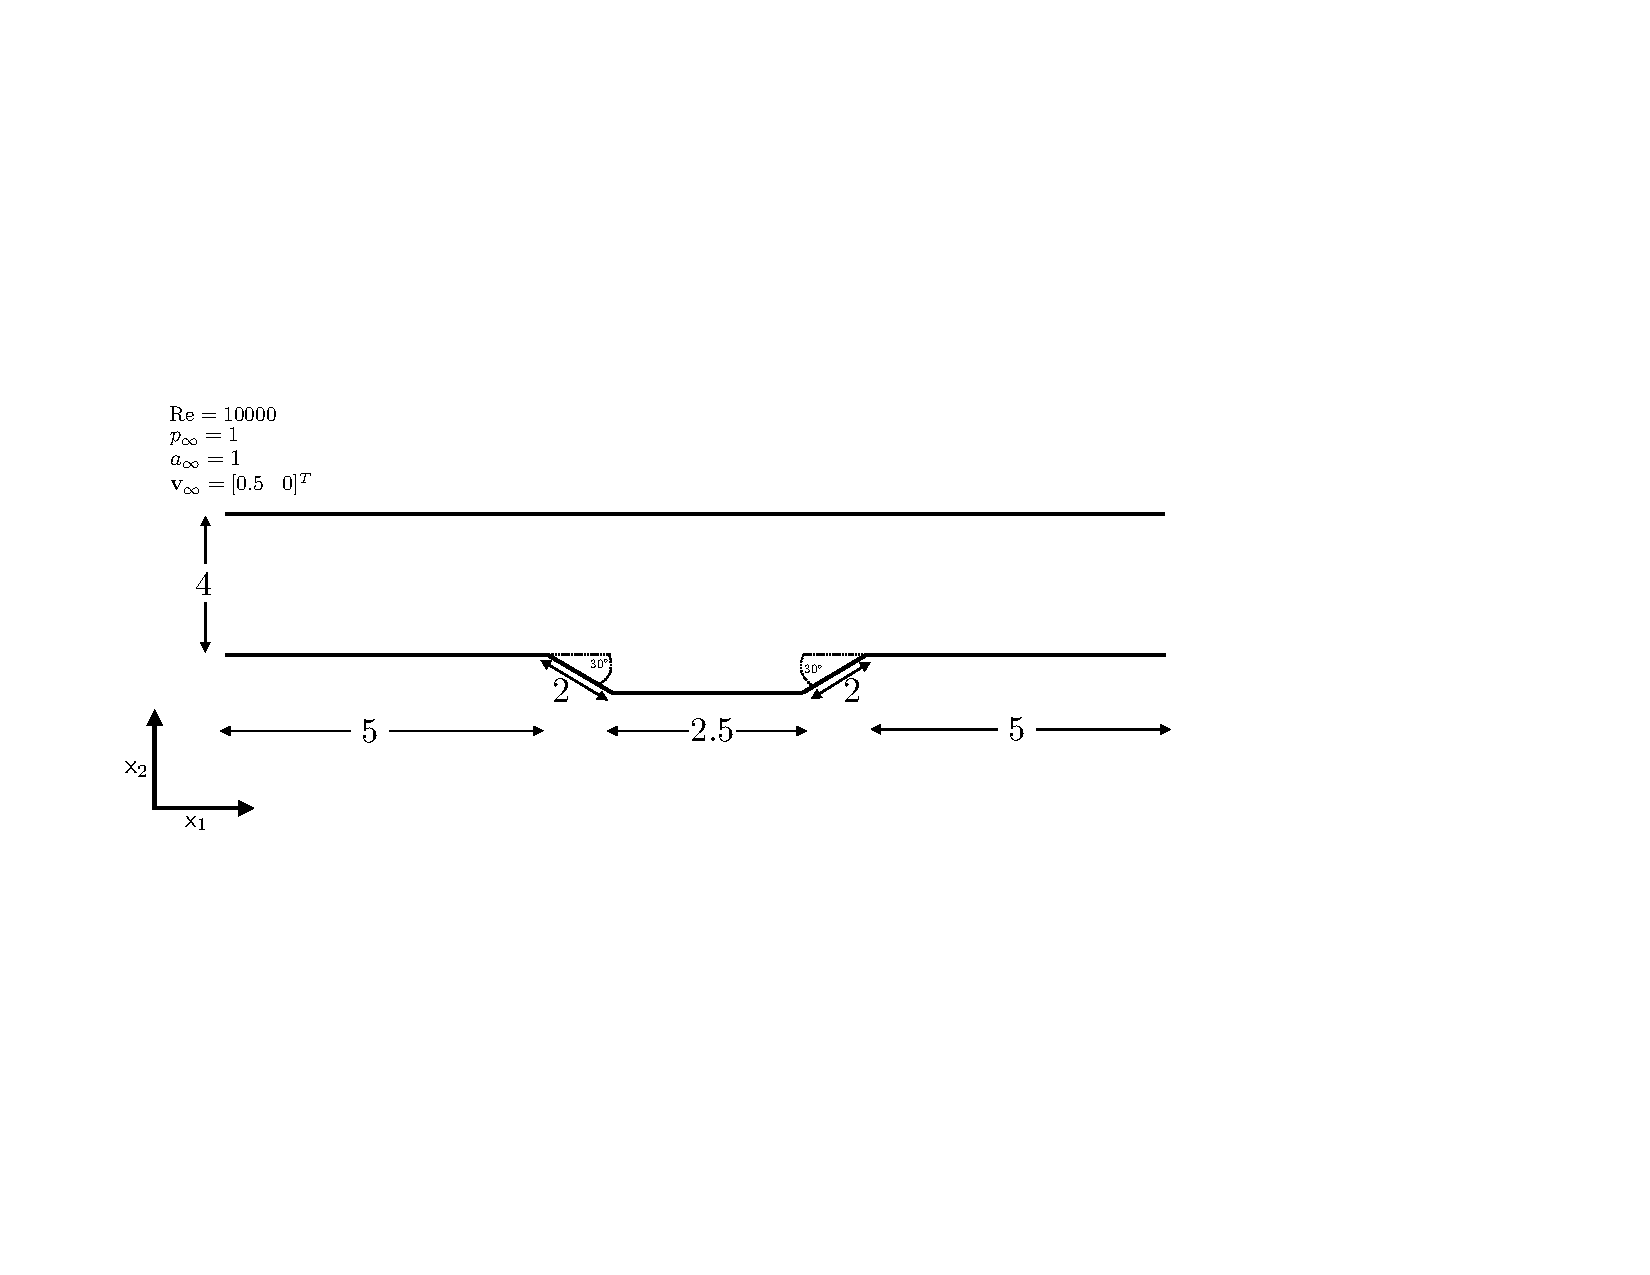
\includegraphics[trim={2cm 7cm 4cm 6cm},clip,width=0.95\linewidth]{cav_fig.pdf}
%\end{subfigure}
\caption{Figure depicting geometry and flow conditions of the cavity flow problem.} 
\label{fig:cav_fig}
\end{center}
\end{figure}

\begin{figure}
\begin{center}
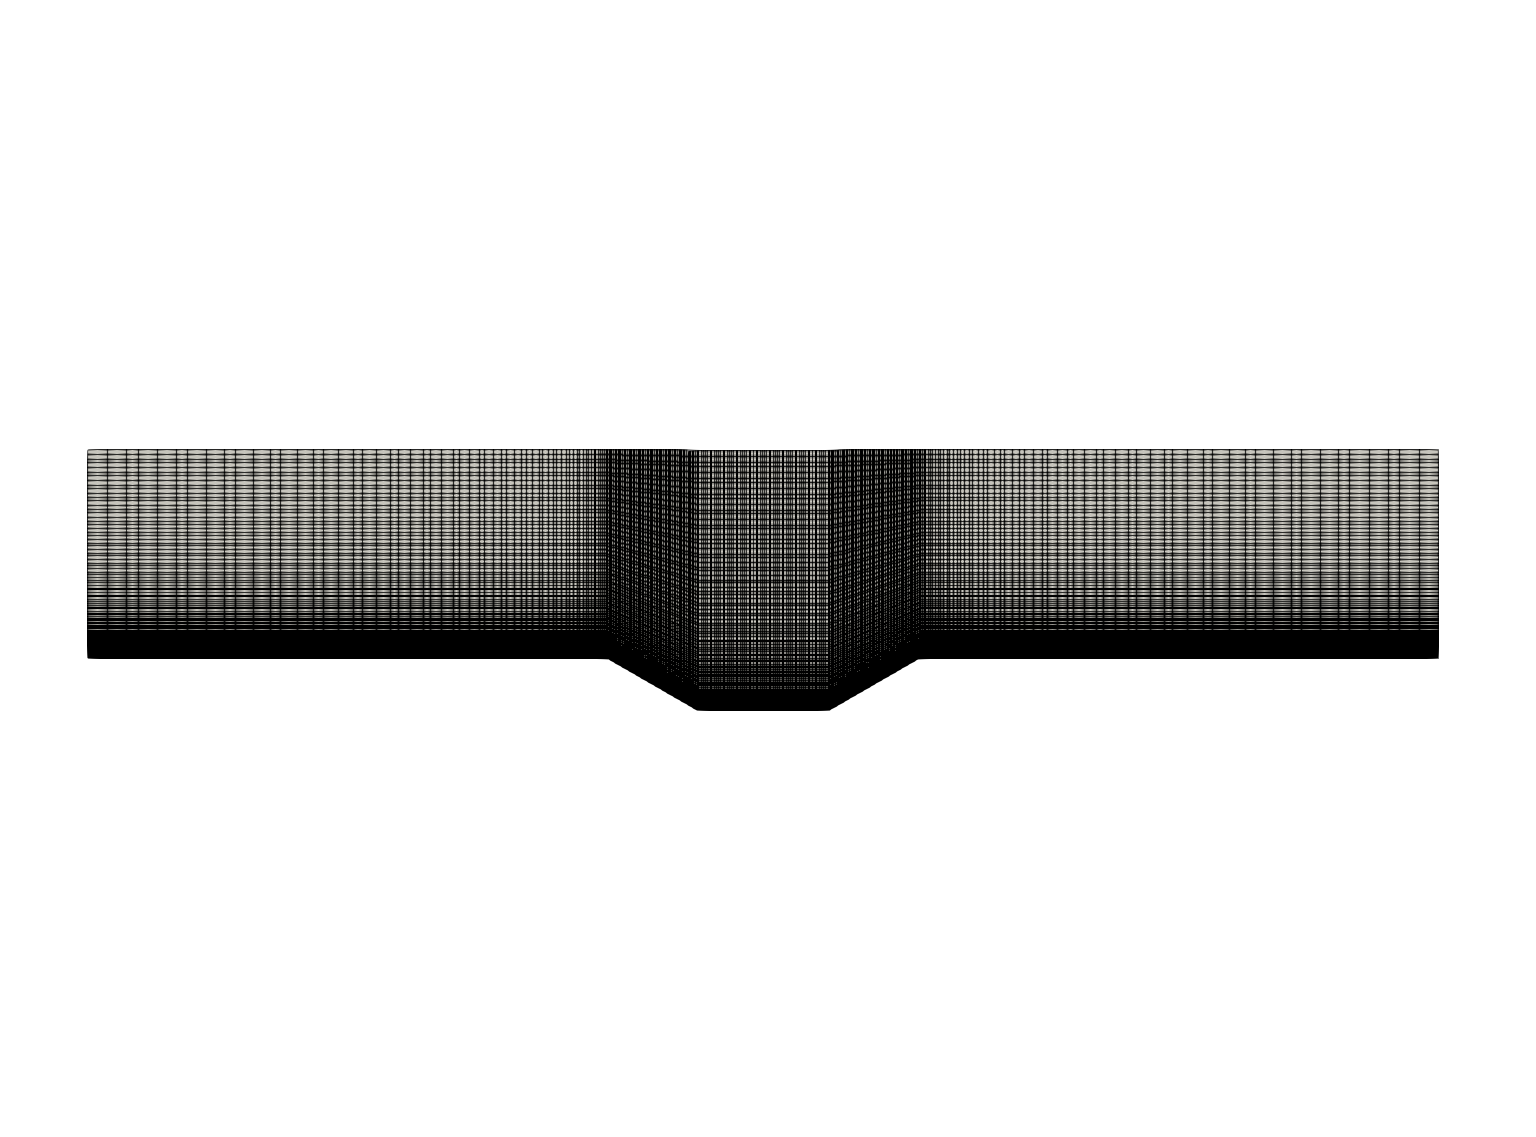
\includegraphics[trim={0cm 14cm 0cm 14cm},clip,width=1.\linewidth]{figs/cavity/grid.png}
\caption{Computational mesh employed in cavity flow simulations.}
\label{fig:cav_mesh}
\end{center}
\end{figure}

\begin{figure} 
\begin{center}
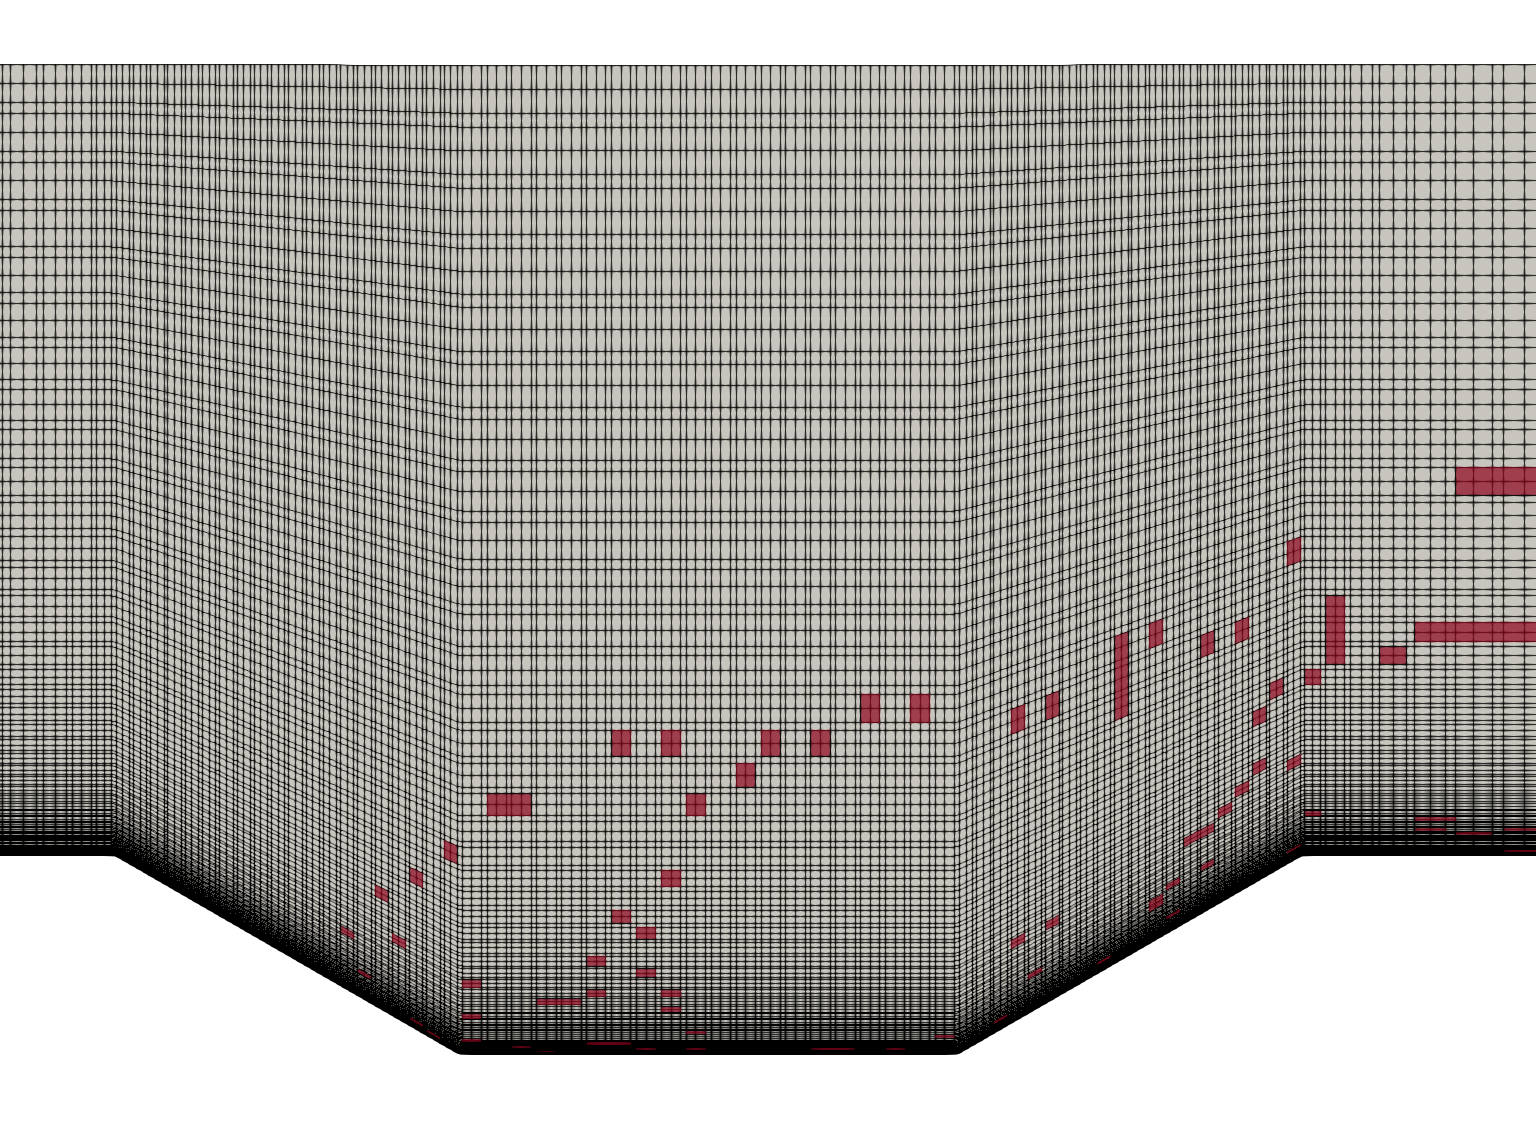
\includegraphics[trim={0cm 0cm 0cm 0cm},clip,width=0.65\linewidth]{figs/cavity/hyper_grid.png}
\caption{Close up of computational mesh with highlighted collocation cells.} 
\label{fig:cav_sampmesh}
\end{center}
\end{figure}

\begin{figure}
\begin{center}
%\begin{subfigure}[t]{0.85\textwidth}
\begin{subfigure}[t]{0.49\textwidth}
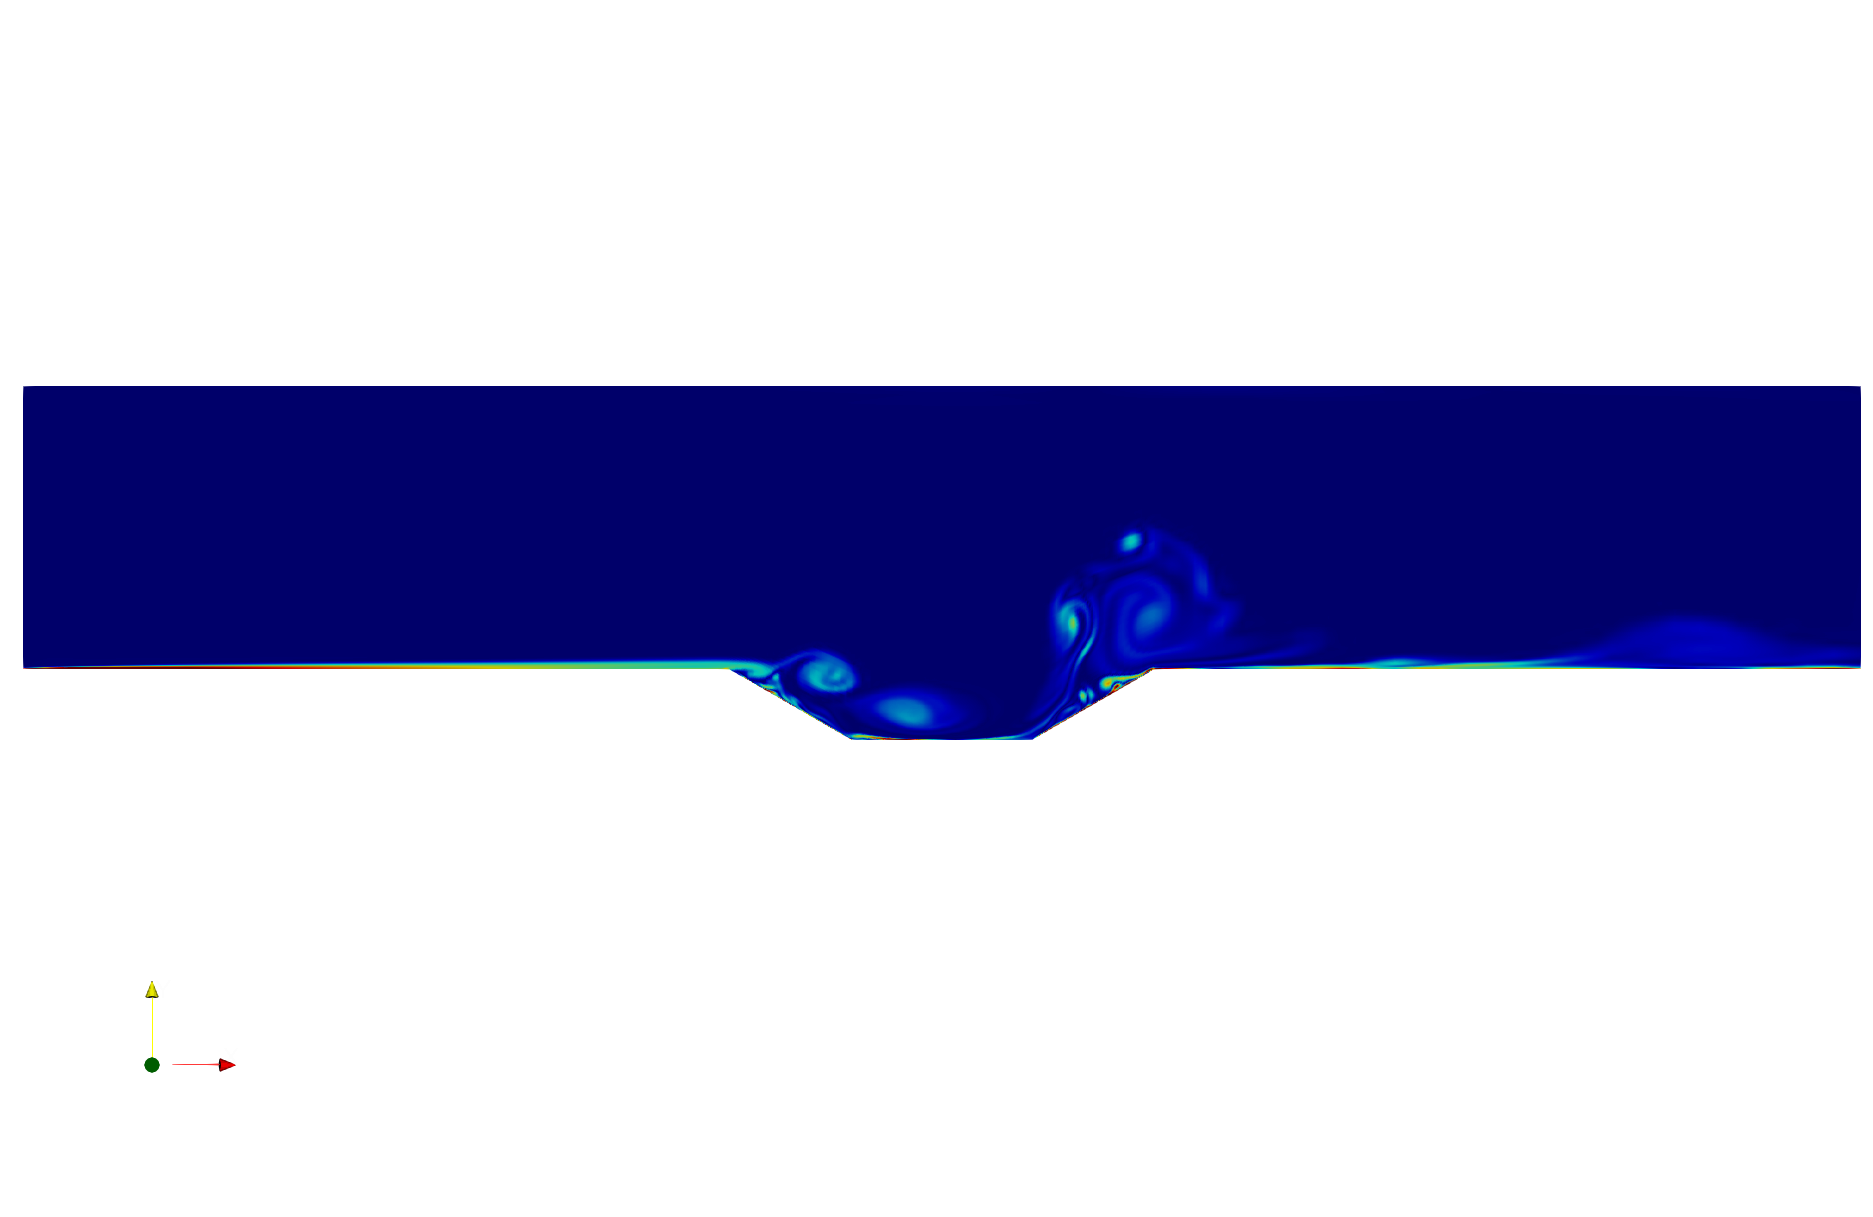
\includegraphics[trim={18cm 16cm 18cm 15cm},clip,width=1.0\linewidth]{figs/cavity/animate/sol0000.png}
\caption{$t=0.0$}
\end{subfigure}
\begin{subfigure}[t]{0.49\textwidth}
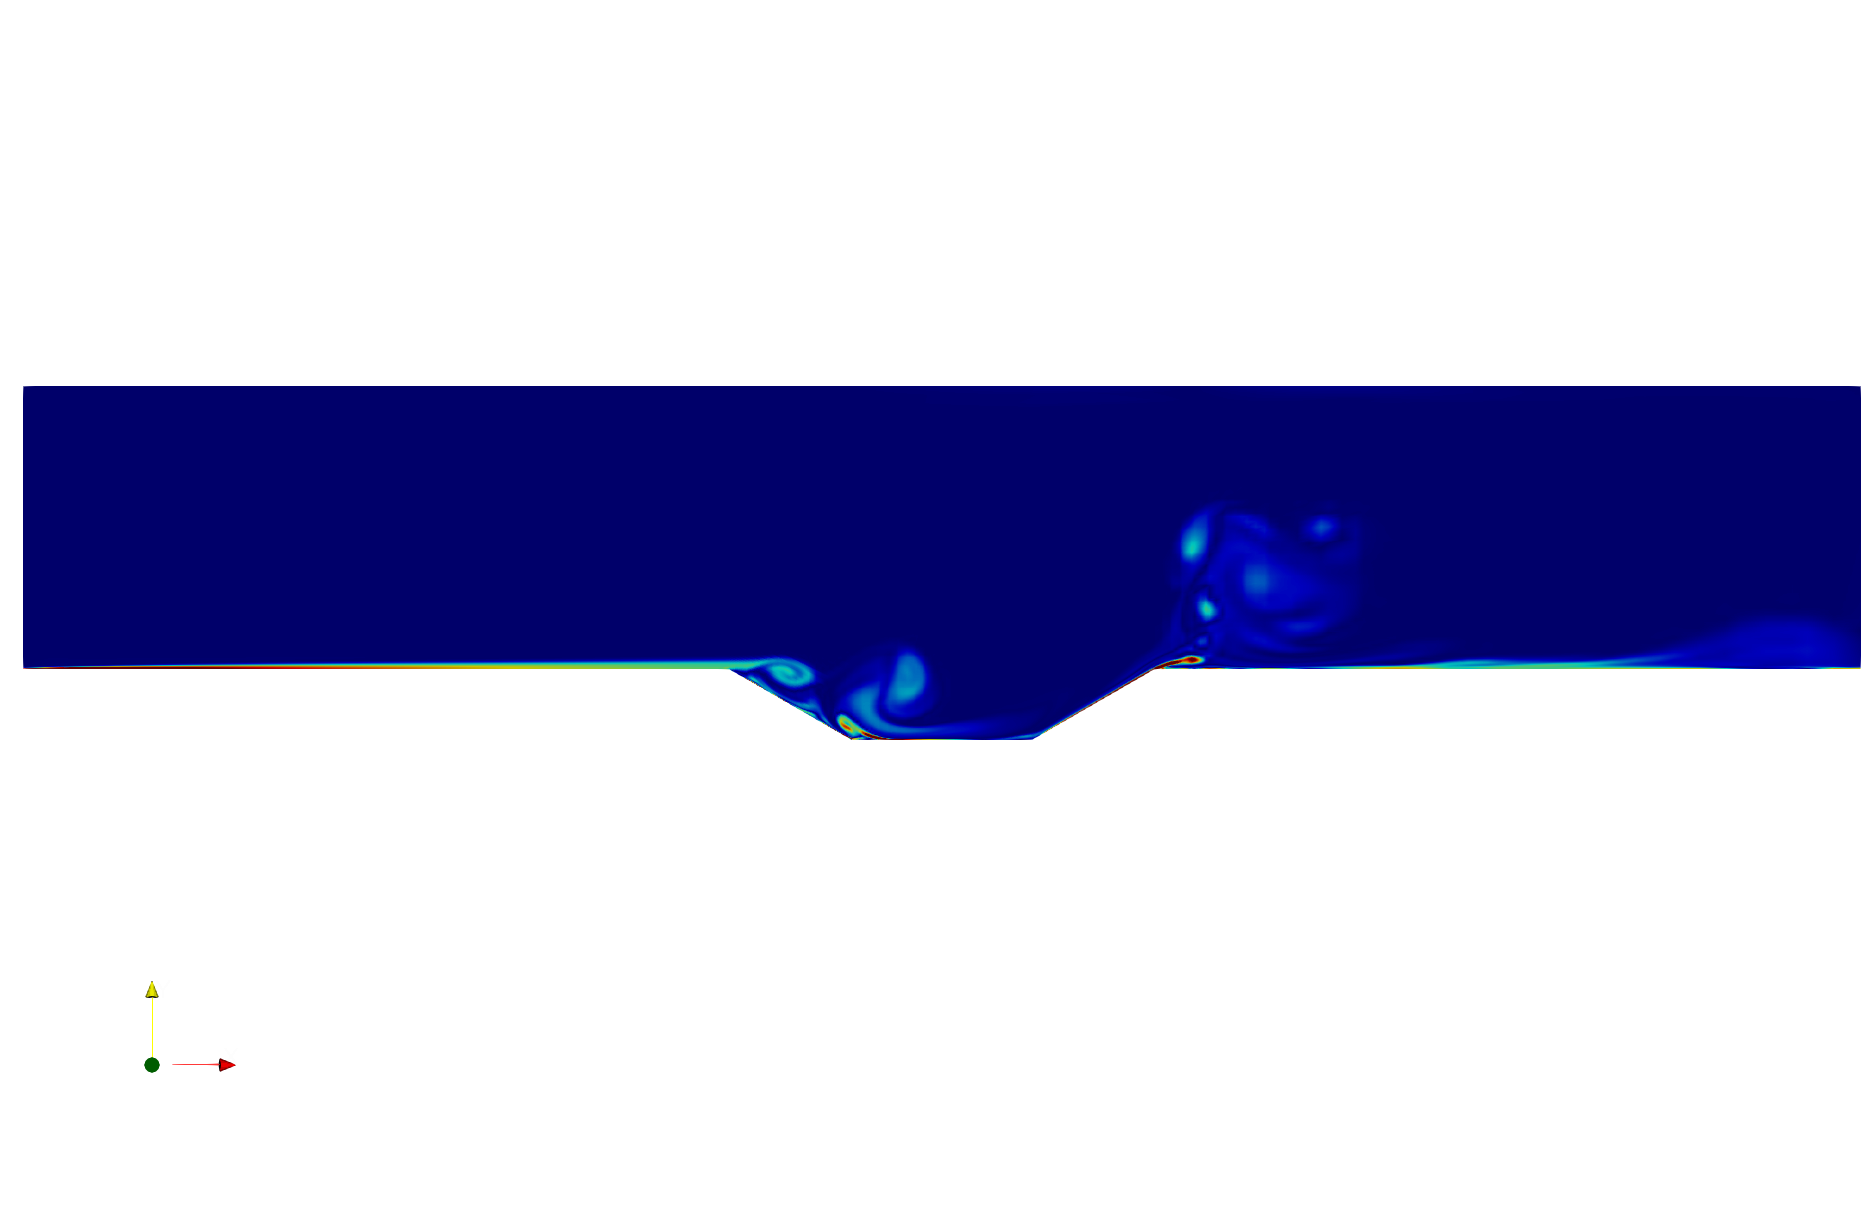
\includegraphics[trim={18cm 16cm 18cm 15cm},clip,width=1.0\linewidth]{figs/cavity/animate/sol0040.png}
\caption{$t=4.0$}
\end{subfigure}
\begin{subfigure}[t]{0.49\textwidth}
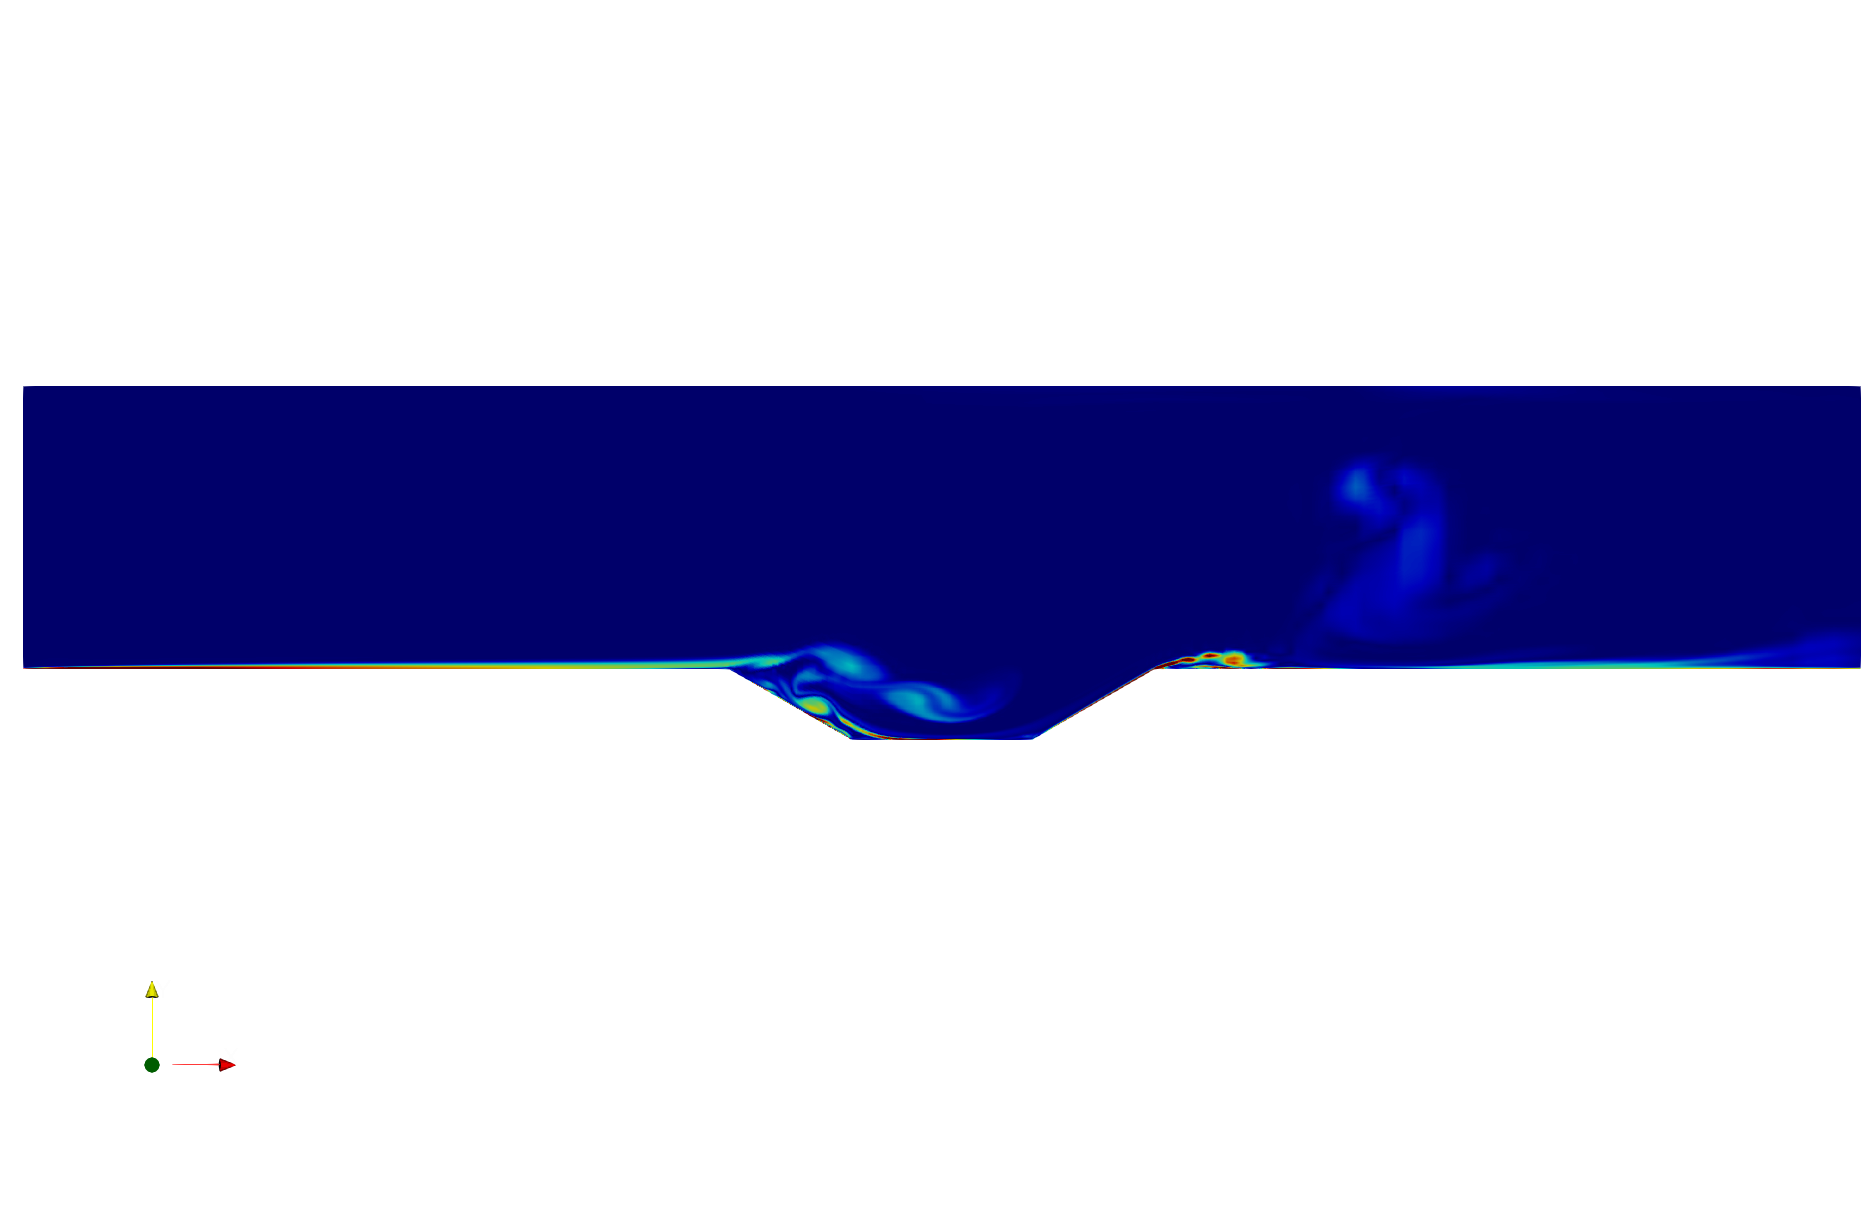
\includegraphics[trim={18cm 16cm 18cm 15cm},clip,width=1.0\linewidth]{figs/cavity/animate/sol0080.png}
\caption{$t=8.0$}
\end{subfigure}
\begin{subfigure}[t]{0.49\textwidth}
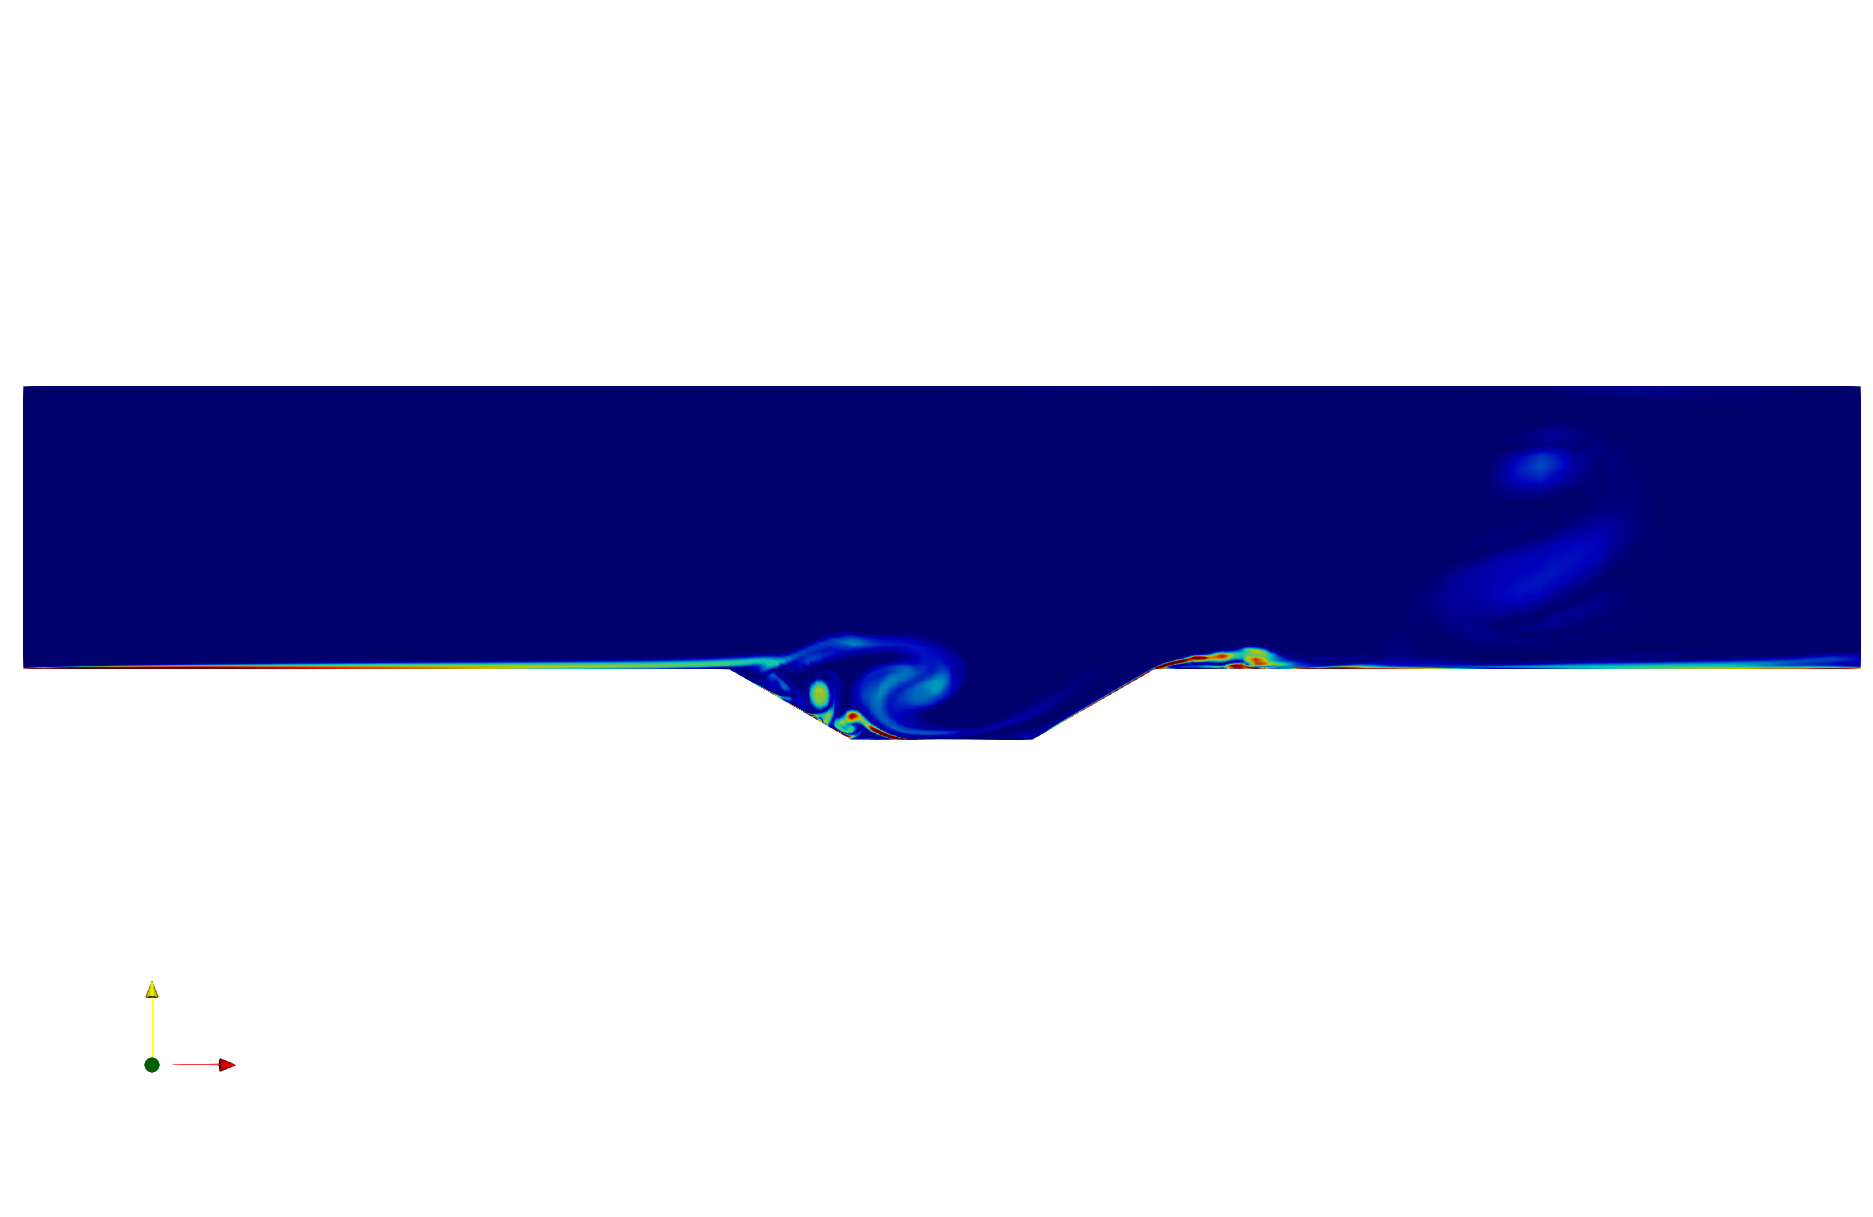
\includegraphics[trim={18cm 16cm 18cm 15cm},clip,width=1.0\linewidth]{figs/cavity/animate/sol0120.png}
\caption{$t=12.0$}
\end{subfigure}
\begin{subfigure}[t]{0.49\textwidth}
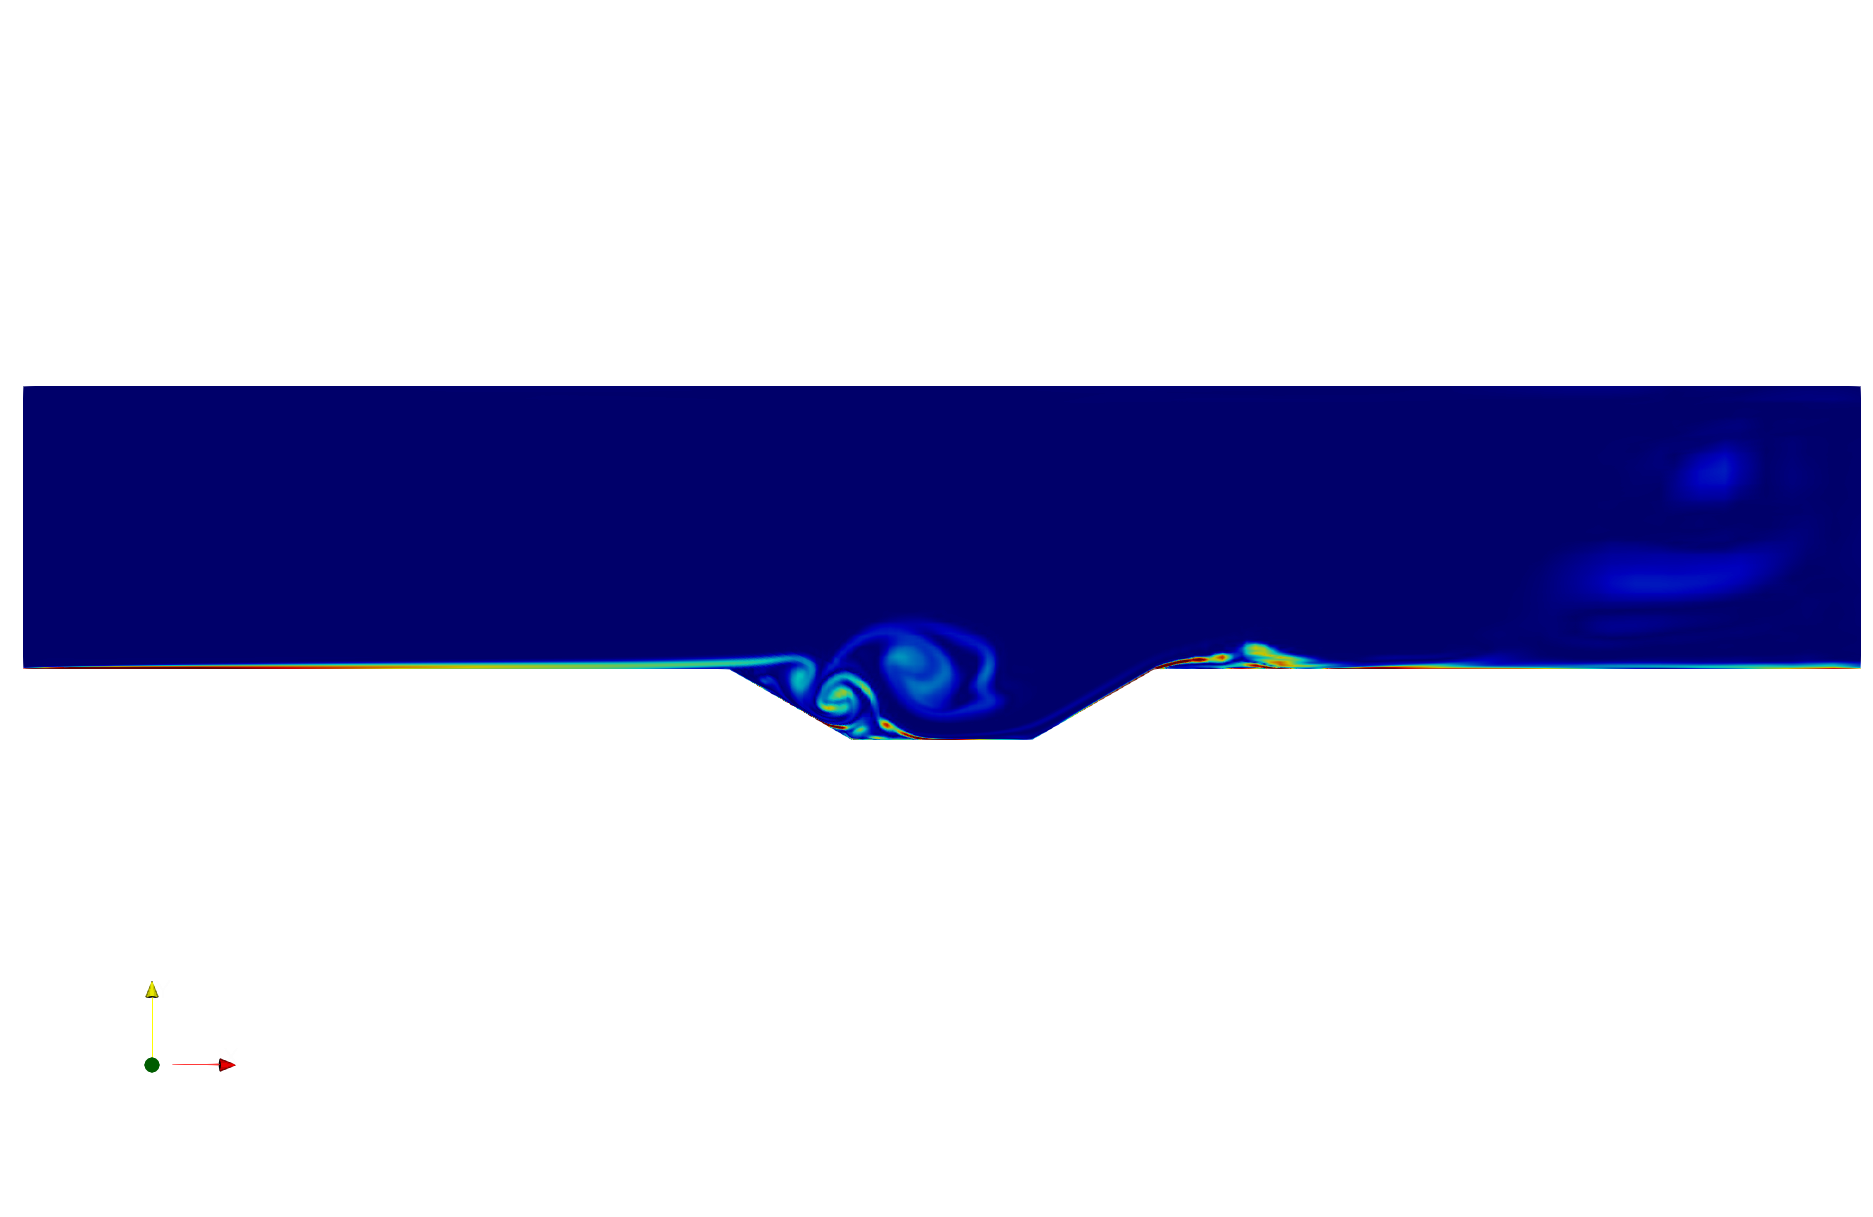
\includegraphics[trim={18cm 16cm 18cm 15cm},clip,width=1.0\linewidth]{figs/cavity/animate/sol0160.png}
\caption{$t=16.0$}
\end{subfigure}
\begin{subfigure}[t]{0.49\textwidth}
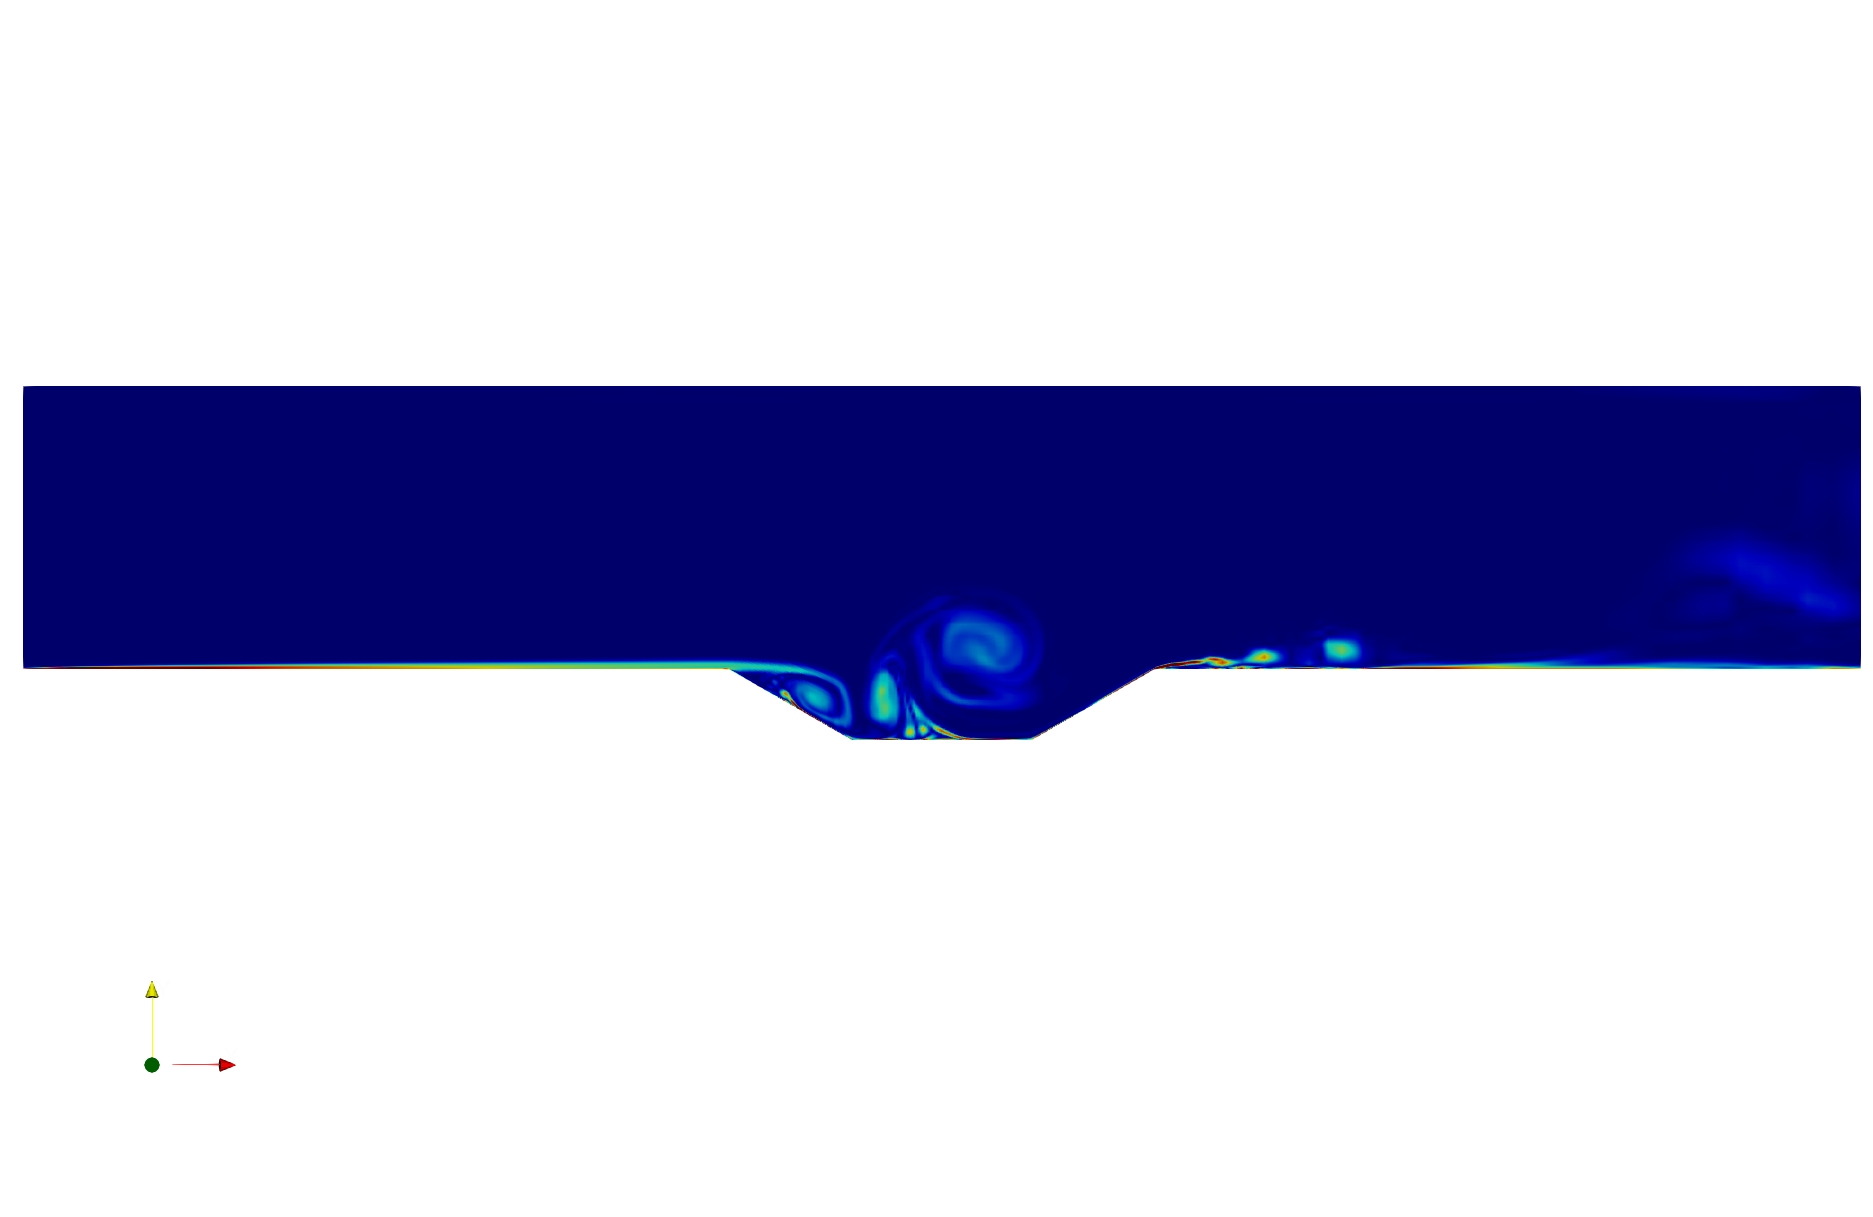
\includegraphics[trim={18cm 16cm 18cm 15cm},clip,width=1.0\linewidth]{figs/cavity/animate/sol0200.png}
\caption{$t=20.0$}
\end{subfigure}
\caption{Vorticity snapshots from the FOM simulation at various time instances.} 
\label{fig:fom_sols_cav}
\end{center}
\end{figure}


\subsubsection{Numerical results}
We first assess the performance of \methodAcronymROMs\ with varying window sizes. To this end, we consider \methodAcronymROMs\ with uniform window 
sizes of $\Delta T^n \equiv \Delta T = 0.2,0.5,1.0,$ and $2.0$, along with the Galerkin and LSPG ROMs. We first consider results for basis \#1 as described in 
Table~\ref{tab:rom_basis_details}. For all ROMs, we evolve 
the solution for $t \in [0,100]$. This comprises the same time interval used to construct the trial subspace. First, Figure~\ref{fig:cav_results1a} depicts the evolution of the pressure at the bottom wall in the midpoint of the computational domain, while Figure~\ref{fig:cav_results1b} depicts the evolution of the normalized $\elltwo$ state error of the various reduced-order models. Both the collocated Galerkin and LSPG ROMs blow up/fail to converge within the first several time units. The \methodAcronymROM\ minimizing the residual over a window of size $\Delta T = 0.2$ also fails to converge. The \methodAcronymROMs\ that minimize the residual over window sizes of $\Delta T \ge 0.5$ are seen to all be stable and accurate; the pressure response is well characterized and the normalized state errors are again less than $10\%$. The most notable discrepancy between the \methodAcronymROM\ and FOM solutions is a slight phase difference. 






\begin{figure}
\begin{center}

\begin{subfigure}[t]{0.95\textwidth}
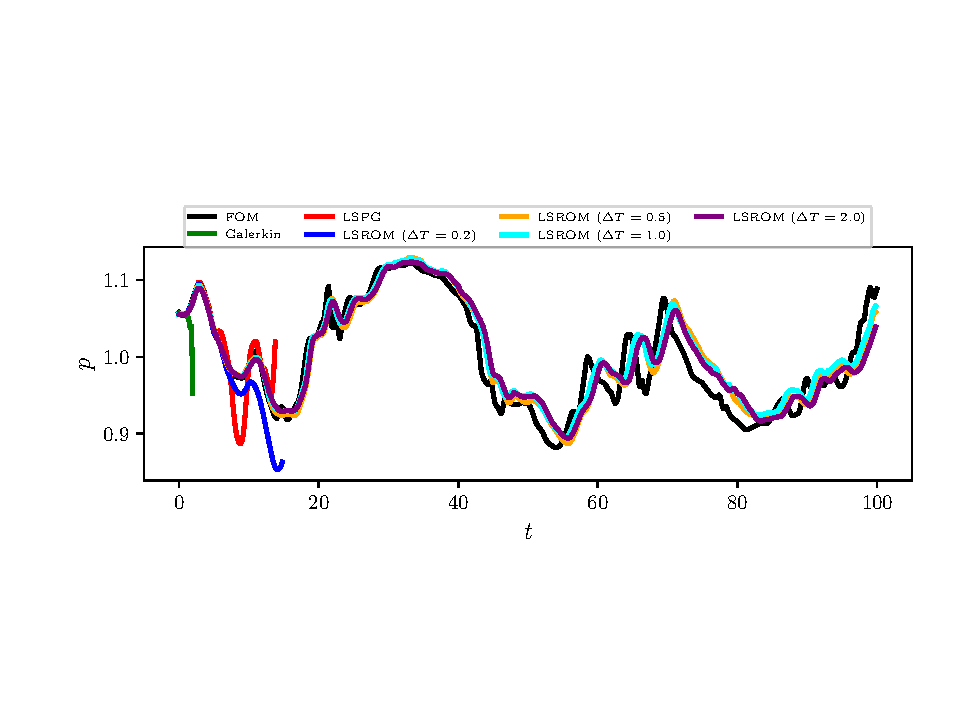
\includegraphics[trim={0cm 3.0cm 0cm 3cm},clip,width=1.\linewidth]{figs/cavity/pressure_basis2.pdf}
\caption{Pressure} 
\label{fig:cav_results1a}
\end{subfigure}

\begin{subfigure}[t]{0.95\textwidth}
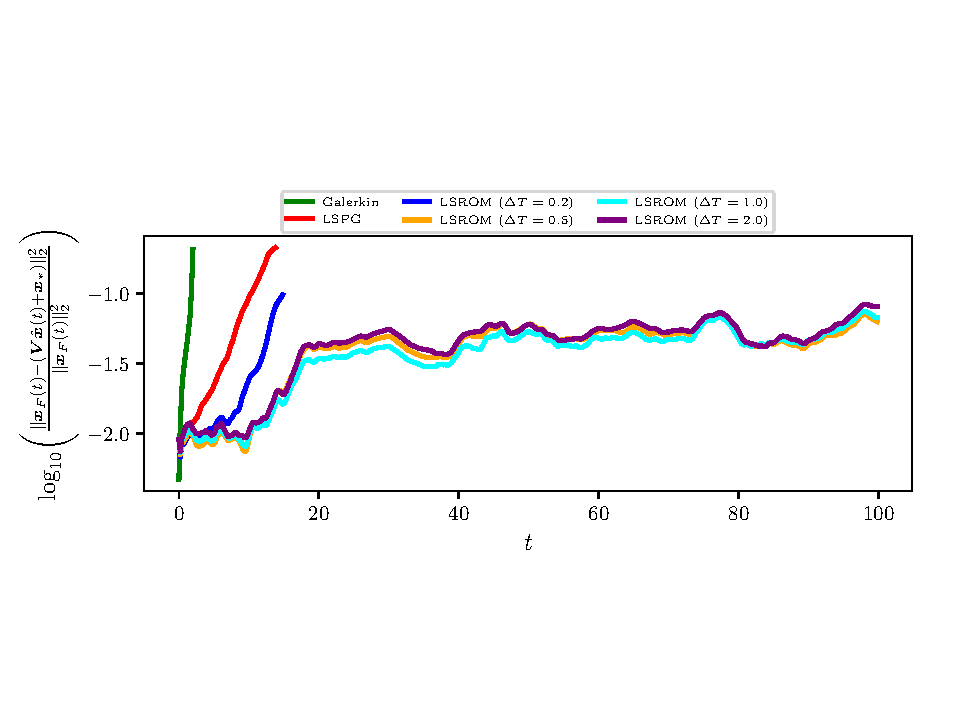
\includegraphics[trim={0cm 2.8cm 0cm 3cm},clip,width=1.\linewidth]{figs/cavity/error_basis2.pdf}
\caption{Normalized $\elltwo$ error}
\label{fig:cav_results1b}
\end{subfigure}

\end{center}
\caption{Comparison of the pressure profiles obtained at the midpoint of the bottom wall (top) and normalized $\elltwo$ state errors (bottom) of various collocated ROMs to the full-order model solution.}
\label{fig:cav_results1}
\end{figure}

Figure~\ref{fig:cav_results2} shows the space--time error and objective function of the stable \methodAcronymROMs. It is seen that growing the window size over 
which the residual is minimized leads to a lower space--time residual, but not necessarily a lower $\elltwo$ error. This result is consistent with the previous numerical example. Next, Figure~\ref{fig:cav_wallclock}
shows the wall-clock times of the \methodAcronymROMs\ for $t \in [0,10]$ as compared to the LSPG ROM\footnote{Note that LSPG blew up at $t \approx 16.0$, so we focus on the first ten time units.}. As expected, increasing $\Delta T$ again leads to an increase in computational cost; minimizing the residual over a window comprising 20 time instances yields a 2.5x increase in cost over LSPG. 


\begin{figure}
\begin{center}
\begin{subfigure}[t]{0.45\textwidth}
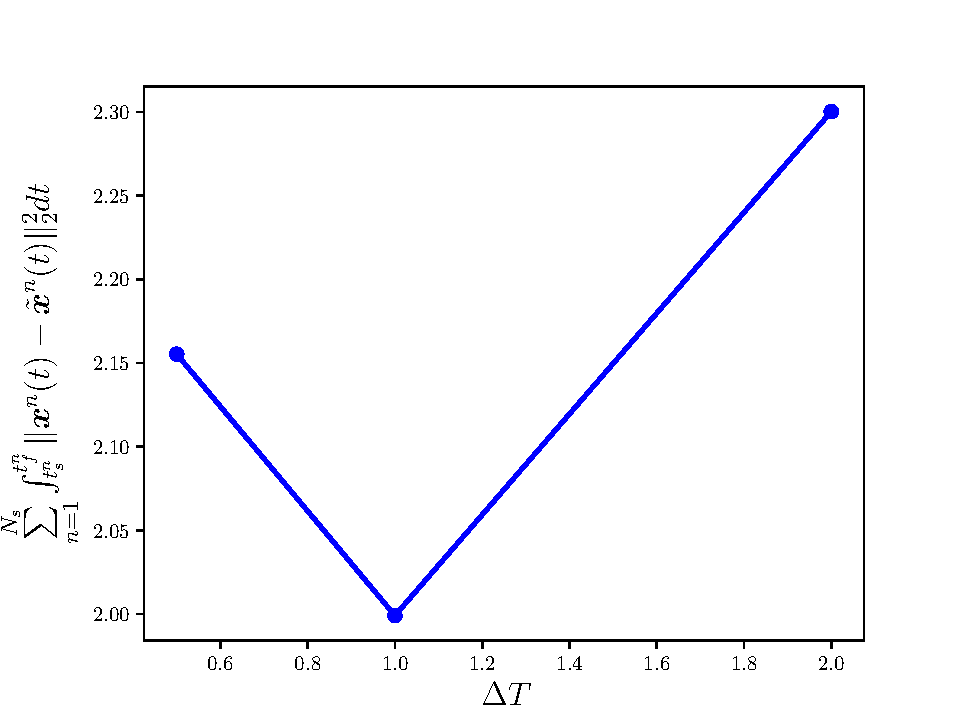
\includegraphics[trim={0cm 0cm 0cm 0cm},clip,width=1.\linewidth]{figs/cavity/error_vs_window_basis2.pdf}
\caption{Space--time $\elltwo$ error}
\label{fig:cav_results2a}
\end{subfigure}
\begin{subfigure}[t]{0.45\textwidth}
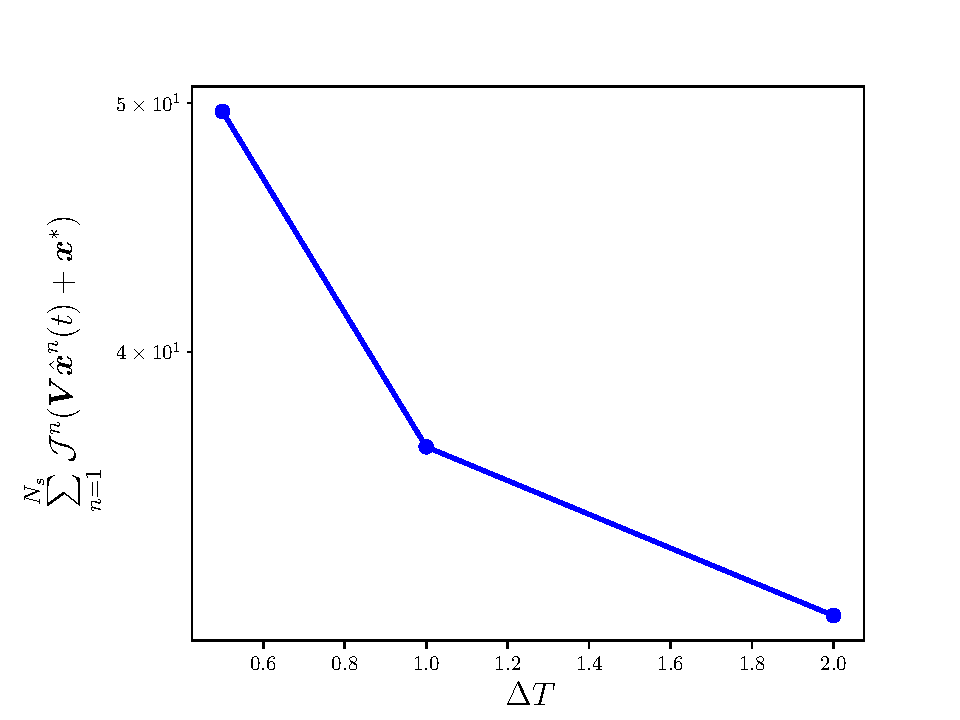
\includegraphics[trim={0cm 0cm 0cm 0cm},clip,width=1.\linewidth]{figs/cavity/objective_vs_window_basis2.pdf}
\caption{Objective function} 
\label{fig:cav_results2b}
\end{subfigure}
\end{center}
\caption{Space--time error (left) and objective function (right) as a function of window size.}
\label{fig:cav_results2}
\end{figure}


\begin{figure}
\begin{center}
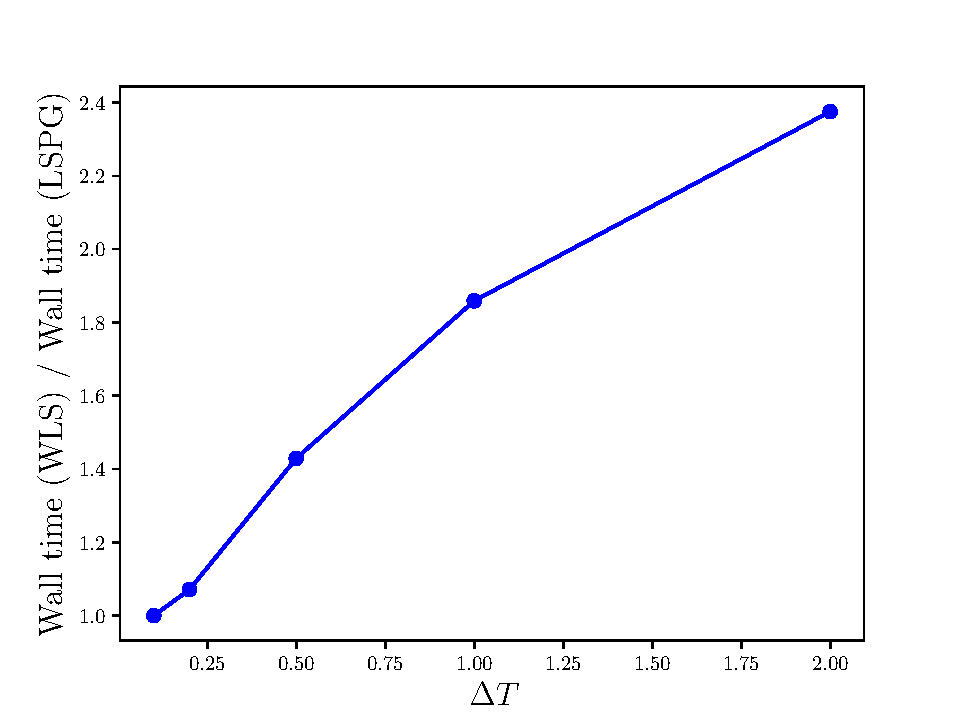
\includegraphics[trim={0cm 0cm 0cm 0cm},clip,width=0.49\linewidth]{figs/cavity/walltime_vs_window_compare_basis2.pdf}
\caption{Wall-clock times of \methodAcronymROMs\ with respect to the LSPG ROM.}
\label{fig:cav_wallclock}
\end{center}
\end{figure}

Figure~\ref{fig:cav_snapshots} shows vorticity fields for the FOM, LSPG ROM, and \methodAcronymROM\ with $\Delta T = 0.5$ for the time instance $t = 5.0$. LSPG is observed to exhibit artificial oscillations; the Gauss-Newton method fails to converge at $t \approx 16.0$. The \methodAcronymROM\ at $\Delta T = 0.5$ is able to capture the important features of the flow, including the points of flow separation at the start and end of the ramp, and remains stable for the entire time interval.  

\begin{figure}
\begin{center}
\begin{subfigure}[t]{0.95\textwidth}
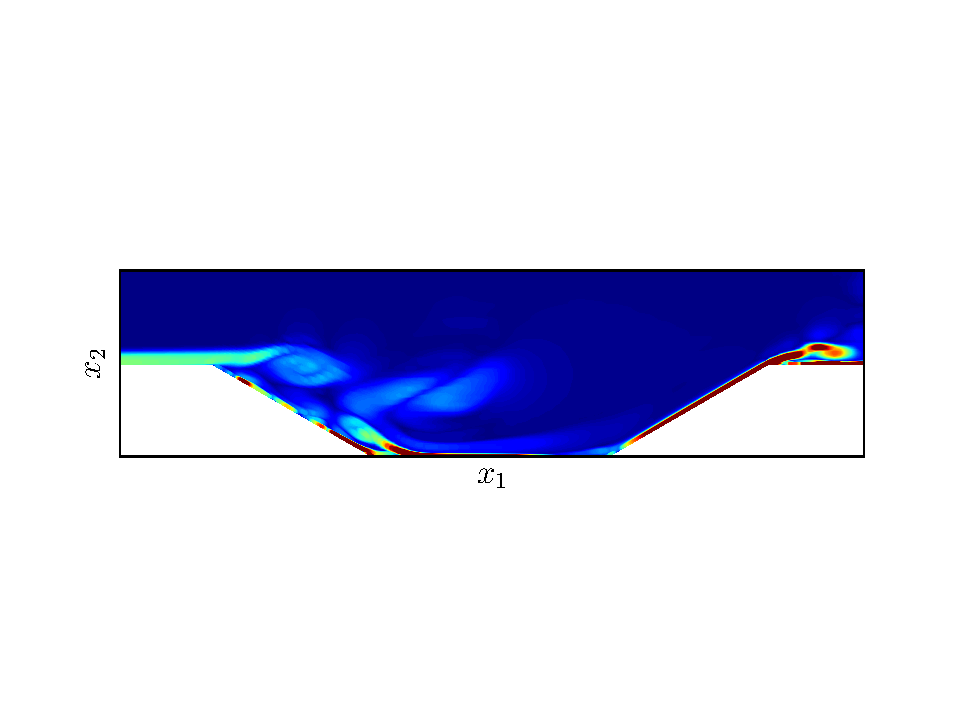
\includegraphics[trim={0cm 3.9cm 0cm 3.9cm},clip,width=1.\linewidth]{figs/cavity/u_fom_t5_basis2.pdf}
\caption{FOM} 
\end{subfigure}
%\begin{subfigure}[t]{0.95\textwidth}
%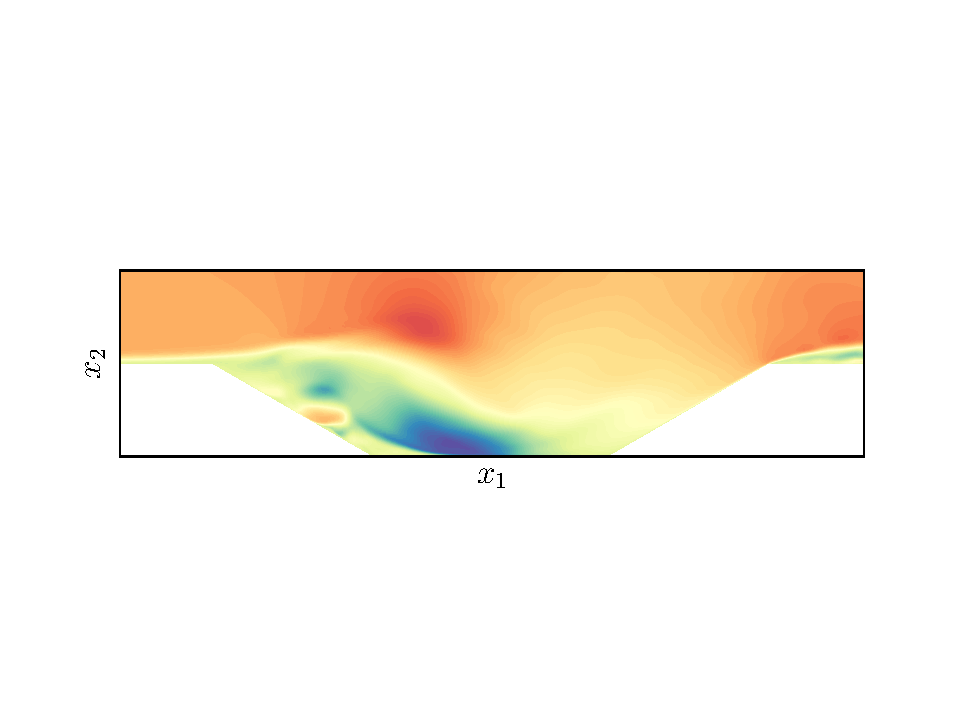
\includegraphics[trim={0cm 3.9cm 0cm 3.9cm},clip,width=1.\linewidth]{figs/cavity/u_c2_t10.pdf}
%\caption{\methodAcronym, $\Delta T = 0.2$} 
%\end{subfigure}
\begin{subfigure}[t]{0.95\textwidth}
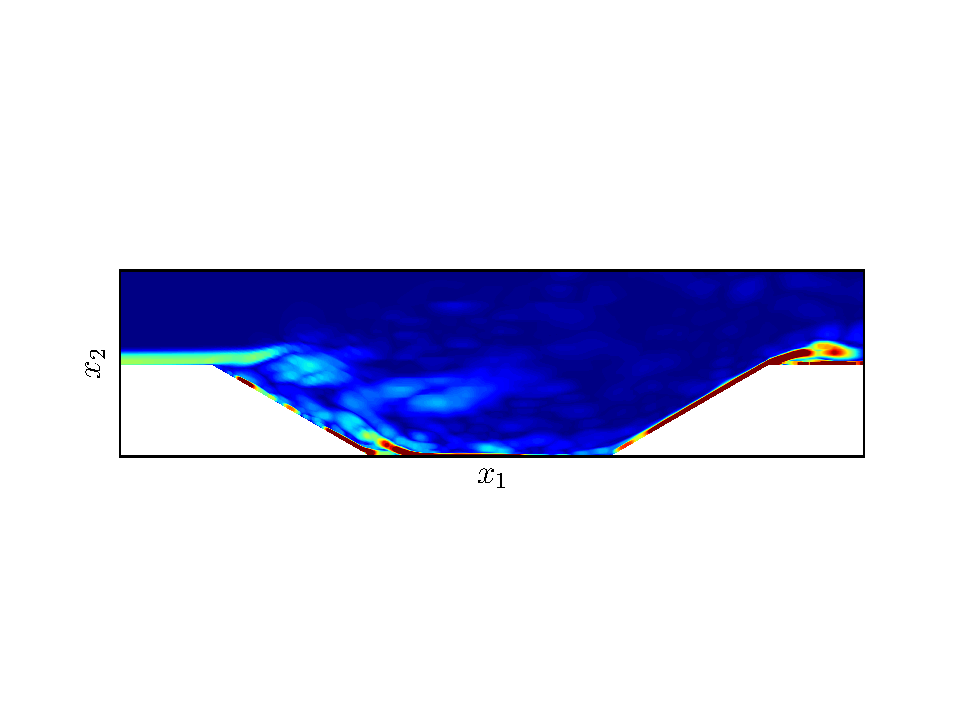
\includegraphics[trim={0cm 3.9cm 0cm 3.9cm},clip,width=1.\linewidth]{figs/cavity/u_lspg_t5_basis2.pdf}
\caption{LSPG} 
\end{subfigure}
\begin{subfigure}[t]{0.95\textwidth}
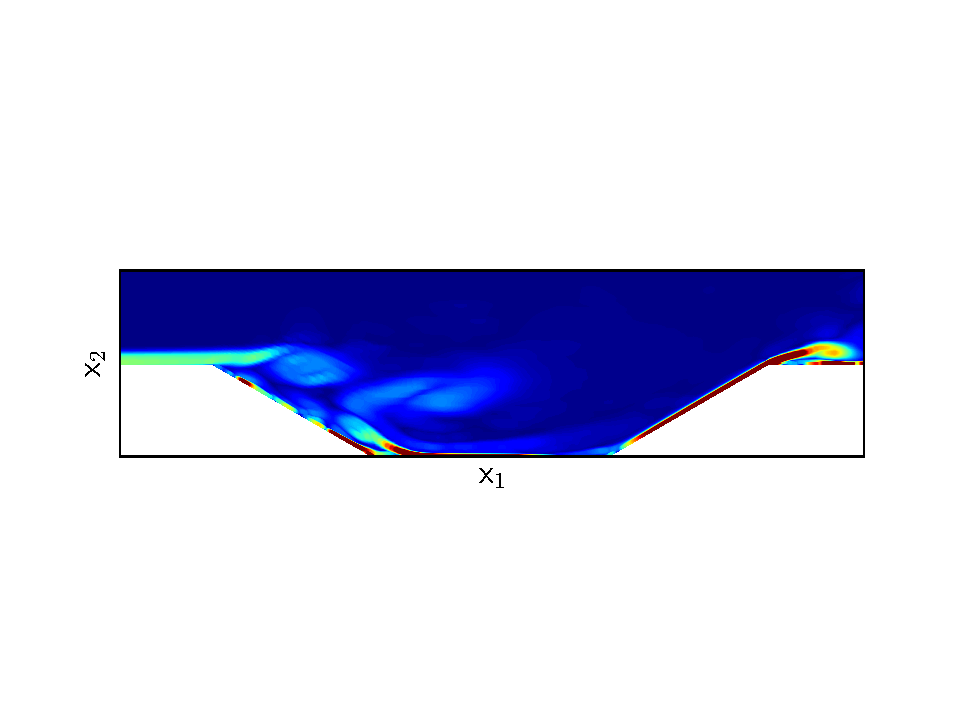
\includegraphics[trim={0cm 3.9cm 0cm 3.9cm},clip,width=1.\linewidth]{figs/cavity/u_c5_t5_basis2.pdf}
\caption{\methodAcronym, $\Delta T = 0.5$} 
\end{subfigure}
%\begin{subfigure}[t]{0.95\textwidth}
%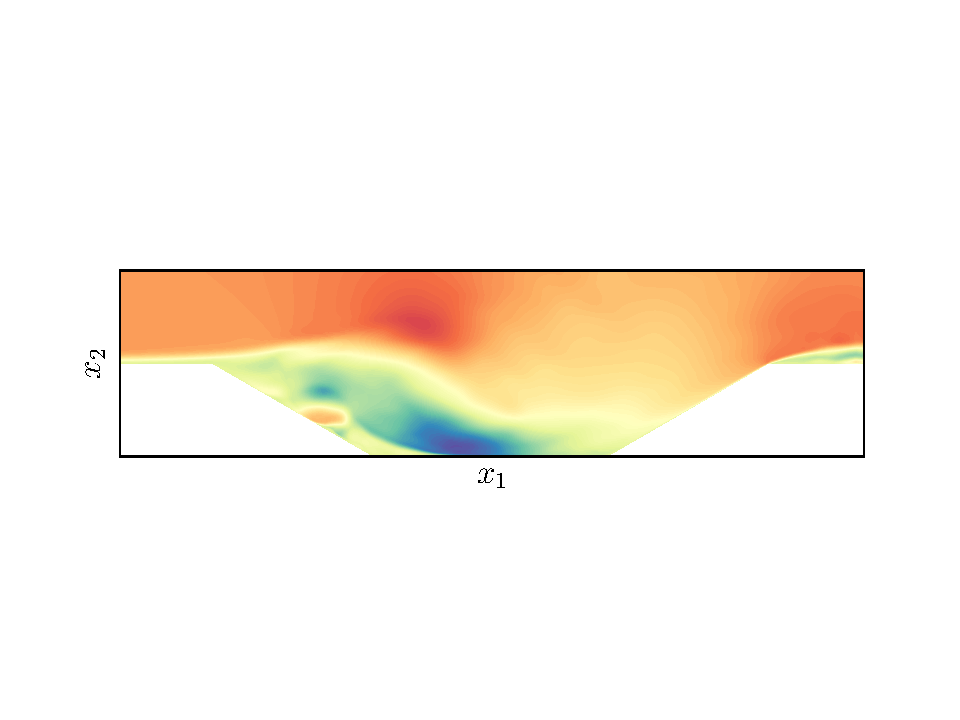
\includegraphics[trim={0cm 3.9cm 0cm 3.9cm},clip,width=1.\linewidth]{figs/cavity/u_c10_t10.pdf}
%\caption{\methodAcronym, $\Delta T = 2.0$} 
%\end{subfigure}
\caption{Field solutions for the vorticity at $t = 5.0$}
\label{fig:cav_snapshots}
\end{center}
\end{figure}


Next, we assess the performance of the various ROMs for basis \#2 as described in Table~\ref{tab:rom_basis_details}, which comprises a richer spatial basis.
 Figure~\ref{fig:cav_results1_basis1} shows the same pressure and error profiles as Figure~\ref{fig:cav_results1}, but for the enriched basis. The LSPG and Galerkin ROMs blow up faster as compared to Figure~\ref{fig:cav_results1}; LSPG fails to converge around $t \approx 8$ (opposed to $t \approx 16$), while Galerkin blows up almost immediately. The 
\methodAcronymROMs\ again yield improved performance: \methodAcronymROMs\ minimizing the residual over window sizes of $\Delta T \ge 0.5$ are seen to all be stable and accurate; the pressure response is well characterized and the normalized state errors are less than $5\%$. The \methodAcronymROMs\ with $\Delta T \ge 0.5$ and basis \#2 yield more accurate results than \methodAcronymROMs\ with basis \#1.
 

\begin{figure}
\begin{center}

\begin{subfigure}[t]{0.95\textwidth}
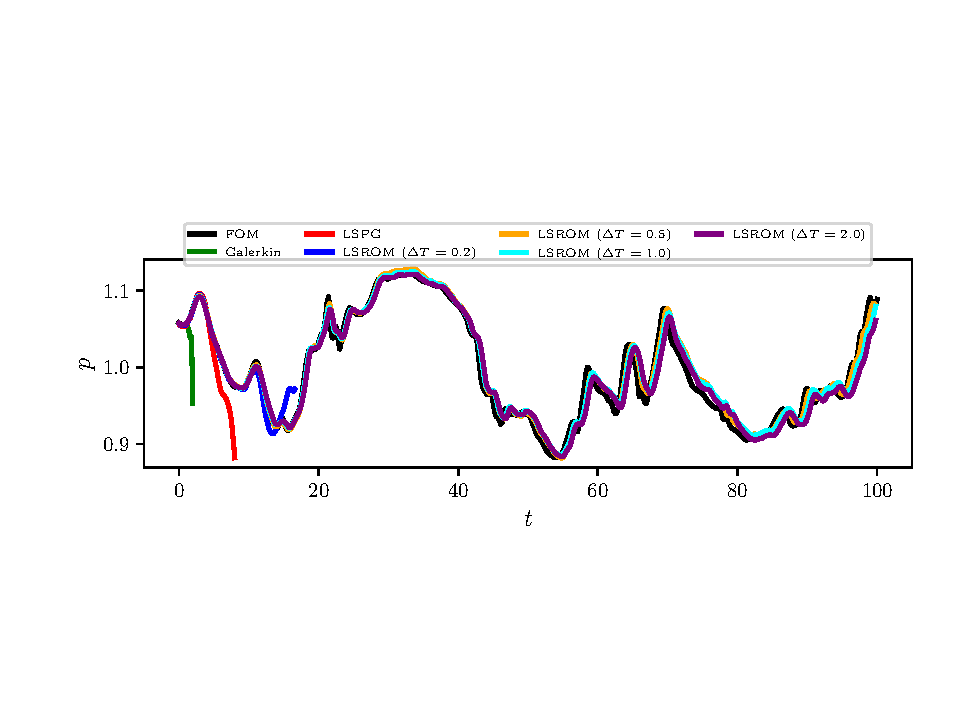
\includegraphics[trim={0cm 2.5cm 0cm 2.5cm},clip,width=1.\linewidth]{figs/cavity/pressure.pdf}
\caption{Pressure} 
\label{fig:cav_results1a_basis1}
\end{subfigure}

\begin{subfigure}[t]{1.0\textwidth}
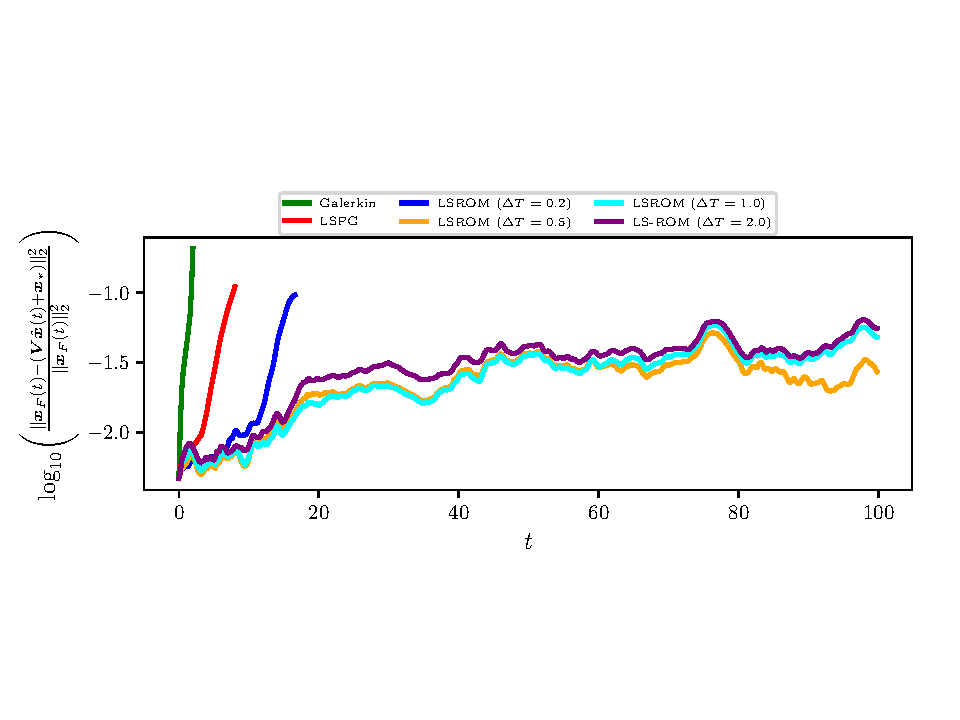
\includegraphics[trim={0cm 2.5cm 0cm 3cm},clip,width=1.\linewidth]{figs/cavity/error.pdf}
\caption{Normalized $\elltwo$ error}
\label{fig:cav_results1b_basis1}
\end{subfigure}
\end{center}
\caption{Comparison of the pressure profiles obtained at the midpoint of the bottom wall (top) and normalized $\elltwo$ state errors (bottom) of various collocated ROMs to the full-order model solution.}
\label{fig:cav_results1_basis1}
\end{figure}


\begin{figure}
\begin{center}
\begin{subfigure}[t]{0.45\textwidth}
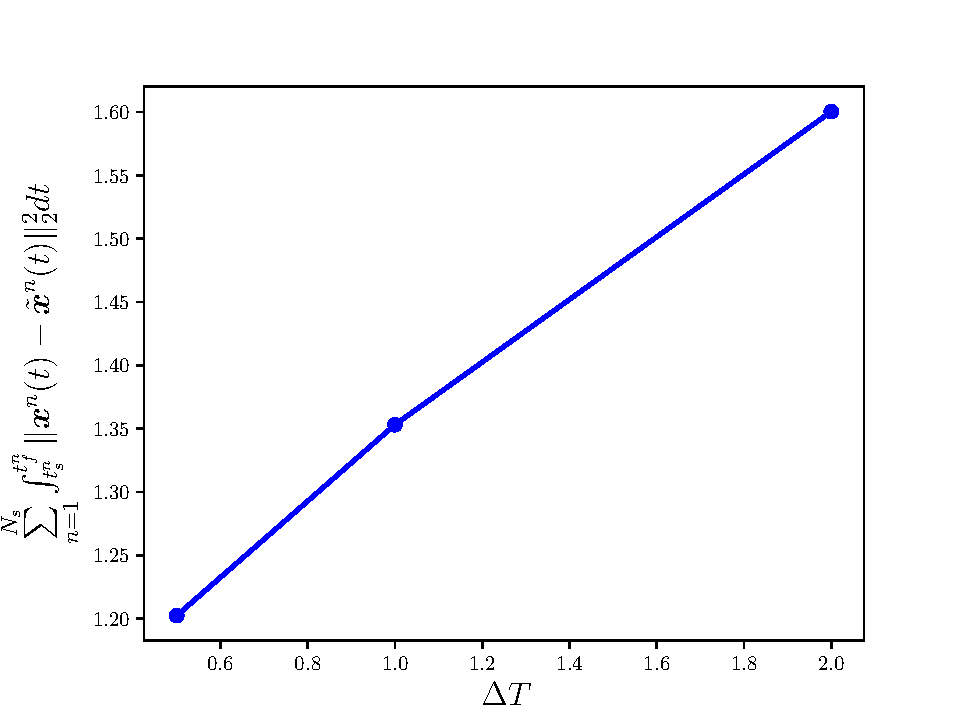
\includegraphics[trim={0cm 0cm 0cm 0cm},clip,width=1.\linewidth]{figs/cavity/error_vs_window.pdf}
\caption{Integrated $\elltwo$ error}
\label{fig:cav_results3a}
\end{subfigure}
\begin{subfigure}[t]{0.45\textwidth}
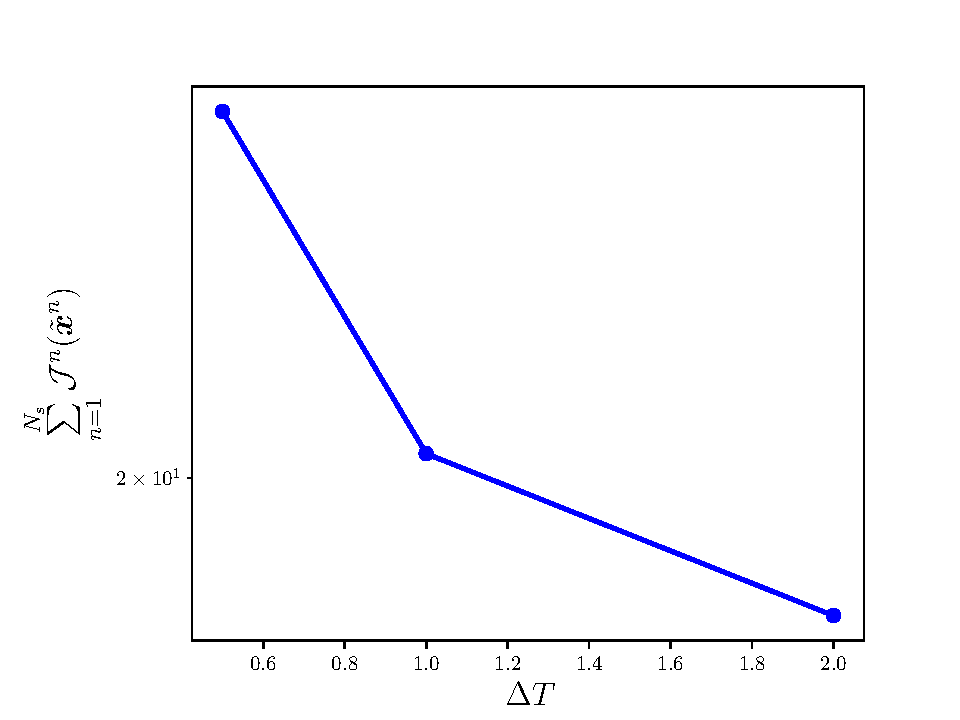
\includegraphics[trim={0cm 0cm 0cm 0cm},clip,width=1.\linewidth]{figs/cavity/objective_vs_window.pdf}
\caption{Objective function} 
\label{fig:cav_results3b}
\end{subfigure}
\end{center}
\caption{Integrated error (left) and objective function (right) as a function of window size.}
\label{fig:cav_results3}
\end{figure}


Finally, Figure~\ref{fig:cav_wallclock} shows the wall-clock times of the \methodAcronymROMs\ as compared to the LSPG ROMs for basis \#2. Increasing the window size again leads to an increase in computational cost. Minimizing the residual over a window comprising 20 time instances yields a 2.5x increase in cost over LSPG. This increase in computational cost is particularly reasonable in this example as LSPG yielded an unstable solution. 
\begin{figure}
\begin{center}
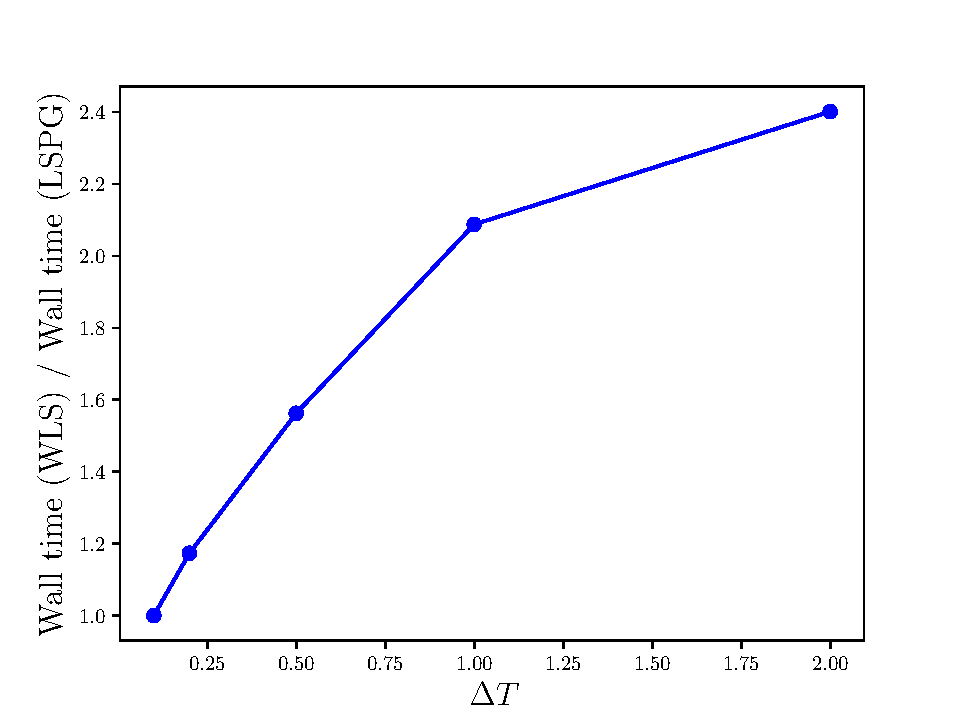
\includegraphics[trim={0cm 0cm 0cm 0cm},clip,width=0.49\linewidth]{figs/cavity/walltime_vs_window_compare.pdf}
\caption{Wall-clock times of \methodAcronymROMs\ with respect to the LSPG ROM.}
\label{fig:cav_wallclock}
\end{center}
\end{figure}


%\begin{figure}
%\begin{center}
%\begin{subfigure}[t]{0.45\textwidth}
%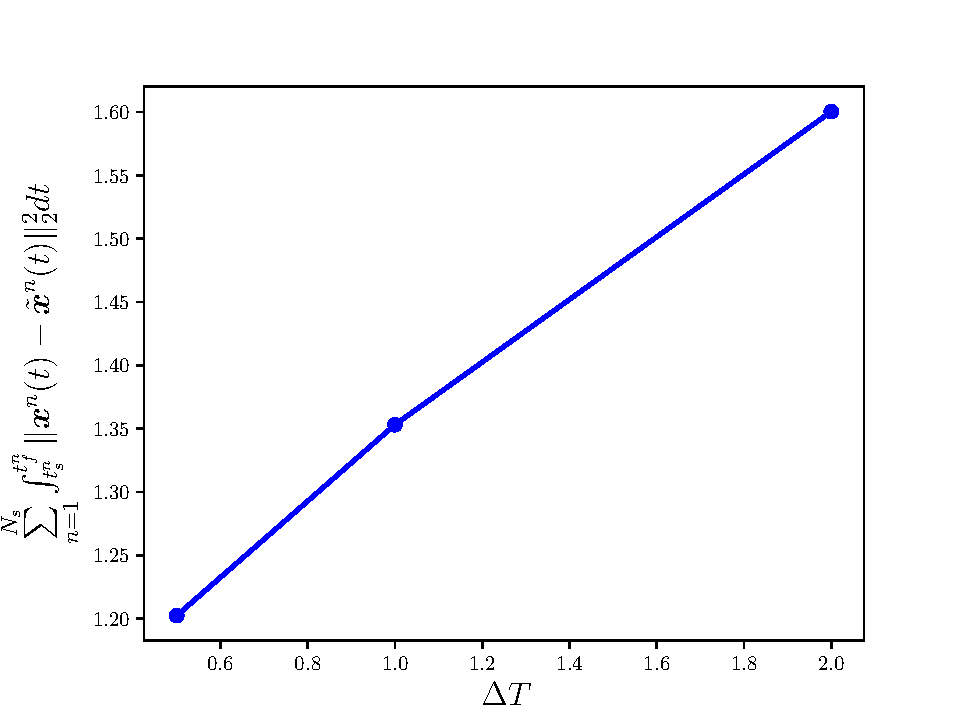
\includegraphics[trim={0cm 0cm 0cm 0cm},clip,width=1.\linewidth]{figs/cavity/error_vs_window.pdf}
%\caption{Integrated $L^2$ error}
%\label{fig:cav_results2a_basis1}
%\end{subfigure}
%\begin{subfigure}[t]{0.45\textwidth}
%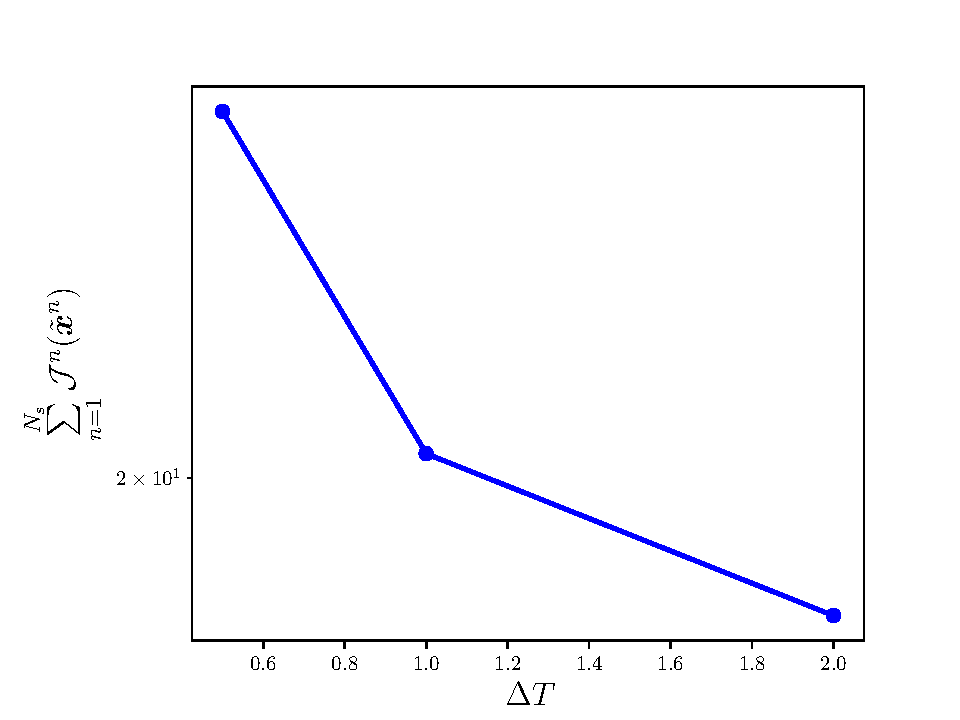
\includegraphics[trim={0cm 0cm 0cm 0cm},clip,width=1.\linewidth]{figs/cavity/objective_vs_window.pdf}
%\caption{Objective function} 
%\label{fig:cav_results2b_basis1}
%\end{subfigure}
%\end{center}
%\caption{Integrated error (left) and objective function (right) as a function of window size.}
%\label{fig:cav_results2_basis1}
%\end{figure}

